\documentclass[11pt,oneside,letterpaper]{article}

% graphicx package, useful for including eps and pdf graphics
\usepackage{graphicx}
\DeclareGraphicsExtensions{.pdf,.png,.jpg}
\include{snippets}
% basic packages
\usepackage{color}
\usepackage{parskip}
\usepackage{float}
\usepackage{subfig}
\usepackage{microtype}
\usepackage{url}
\usepackage[hidelinks]{hyperref}

% text layout
\usepackage{geometry}
\geometry{textwidth=17cm} % 15.25cm for single-space, 16.25cm for double-space
\geometry{textheight=22.5cm} % 22cm for single-space, 22.5cm for double-space

% helps to keep figures from being orphaned on a page by themselves
\renewcommand{\topfraction}{0.85}
\renewcommand{\textfraction}{0.1}

% bold the 'Figure #' in the caption and separate it with a period
% Captions will be left justified
\usepackage[labelfont=bf,labelsep=period,font=small]{caption}

% review layout with double-spacing
%\usepackage{setspace}
%\doublespacing
%\captionsetup{labelfont=bf,labelsep=period,font=doublespacing}

% cite package, to clean up citations in the main text. Do not remove.
\usepackage{cite}
%\renewcommand\citeleft{(}
%\renewcommand\citeright{)}
%\renewcommand\citeform[1]{\textsl{#1}}

% Remove brackets from numbering in list of References
\renewcommand\refname{\large References}
\makeatletter
\renewcommand{\@biblabel}[1]{\quad#1.}
\newcommand{\FIG}[1]{Fig.~\ref{#1}}
\makeatother

\usepackage{authblk}
\renewcommand\Authands{ \& }
\renewcommand\Authfont{\normalsize \bf}
\renewcommand\Affilfont{\small \normalfont}
\makeatletter
\renewcommand\AB@affilsepx{, \protect\Affilfont}
\makeatother

%%% TITLE %%%
\title{\LARGE \bf
Supplementary Information:
The ability of single genes vs full genomes to resolve time and space in outbreak analysis
}

\author[1,2]{Gytis Dudas}
\author[1]{Trevor Bedford}

\affil[1]{Fred Hutchinson Cancer Research Center, Seattle, WA, USA}
\affil[2]{Gothenburg Global Biodiversity Centre, Gothenburg, Sweden}

\date{26 December 2019}
\begin{document}

\maketitle

Citation: Dudas G, Bedford T. 2019. The ability of single genes vs full genomes to resolve time and space in outbreak analysis. BMC Evol Biol 19: 232.

\setcounter{figure}{0}
\setcounter{table}{0}
\renewcommand{\thefigure}{S\arabic{figure}}
\renewcommand{\thetable}{S\arabic{table}}

\begin{figure}[h]
 \centering
	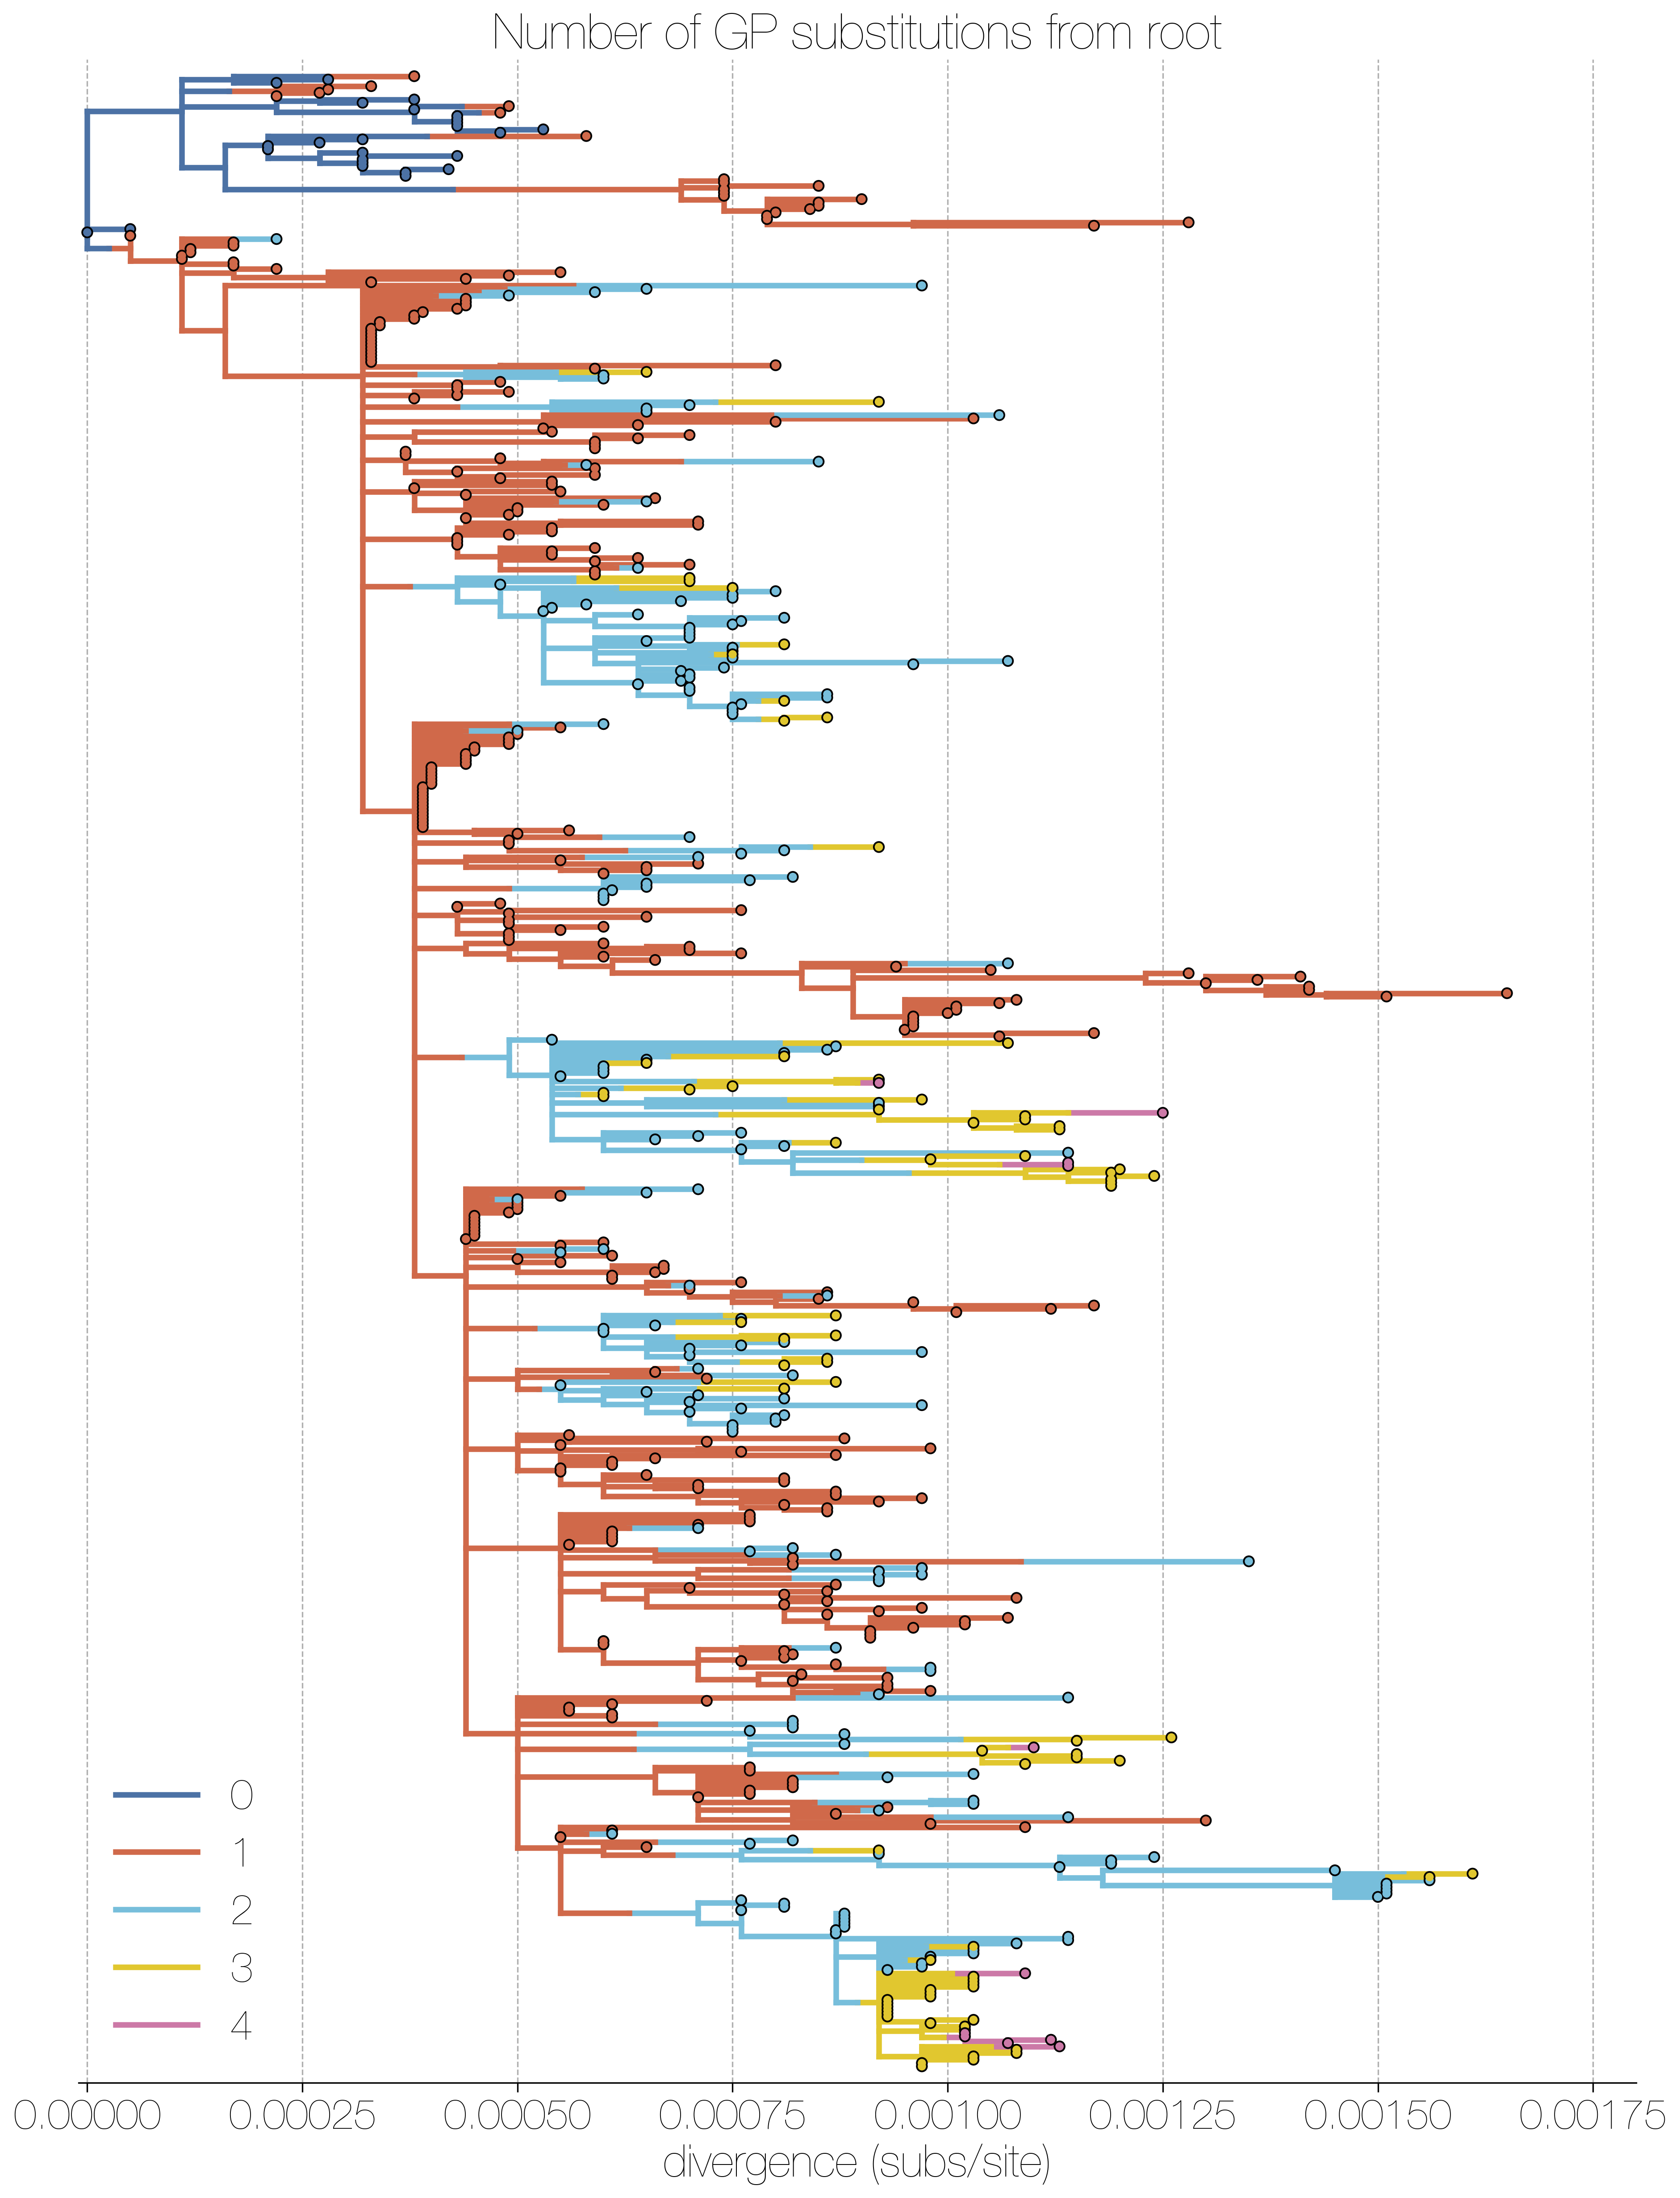
\includegraphics[width=0.75\textwidth]{supp_figures/sfig1_embedding.png}
	\caption{\textbf{Whole genome maximum likelihood tree coloured by mutations occurring in GP.}
  Colours indicate the cumulative number of mutations from the root occurring in the GP gene.
  Much of the clade resolution is lost when only considering mutations occurring in the GP gene, particularly in the already highly polytomic Sierra Leonean part of the phylogeny in red.
	}
	\label{embedding}
\end{figure}

\begin{figure}[h]
 \centering
	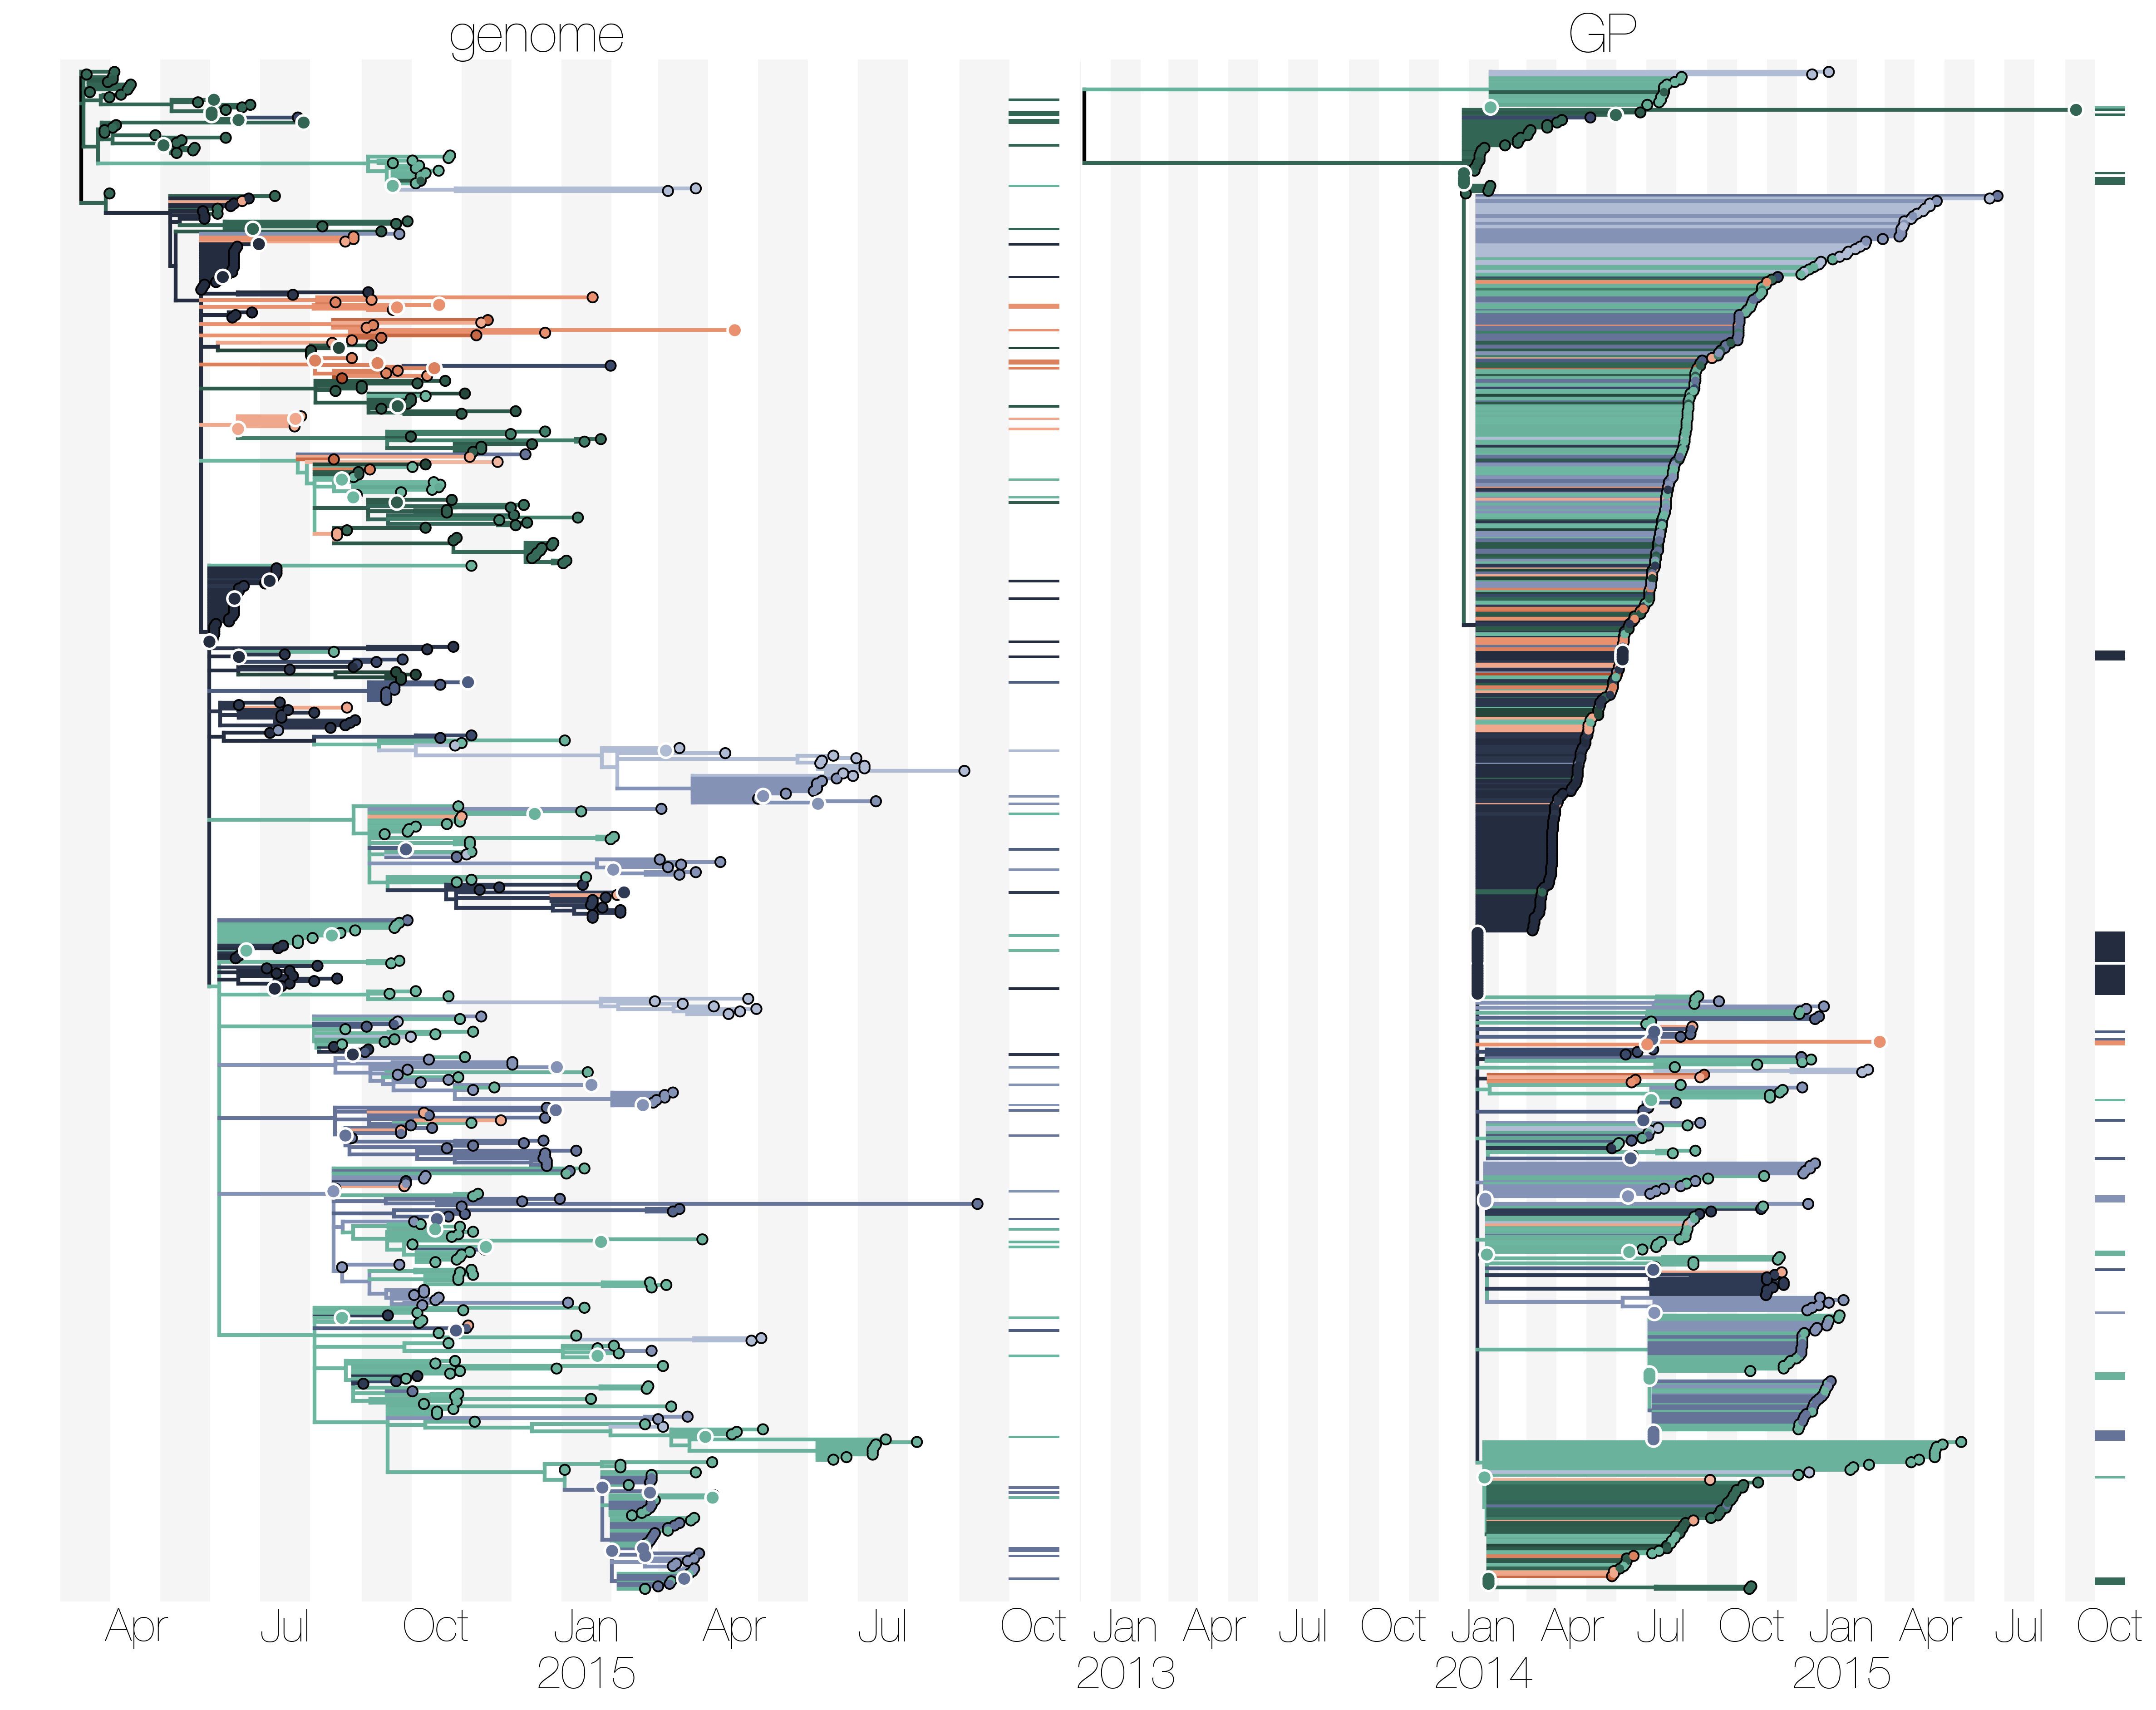
\includegraphics[width=0.75\textwidth]{supp_figures/sfig2_treetimeTrees.png}
	\caption{\textbf{Maximum likelihood phylogenies of complete Ebola virus genomes (left) and GP sequences (right) with maximum likelihood ancestral location reconstruction.}
  Trees were inferred in RAxML with ancestral state reconstruction performed in TreeTime.
  Inferred phylogeographic patterns are for the most part consistent with Bayesian results presented in Figure 1 with severe loss of statistical power when using GP instead of genome sequences.
	}
	\label{TTtrees}
\end{figure}

\begin{figure}[h]
 \centering
	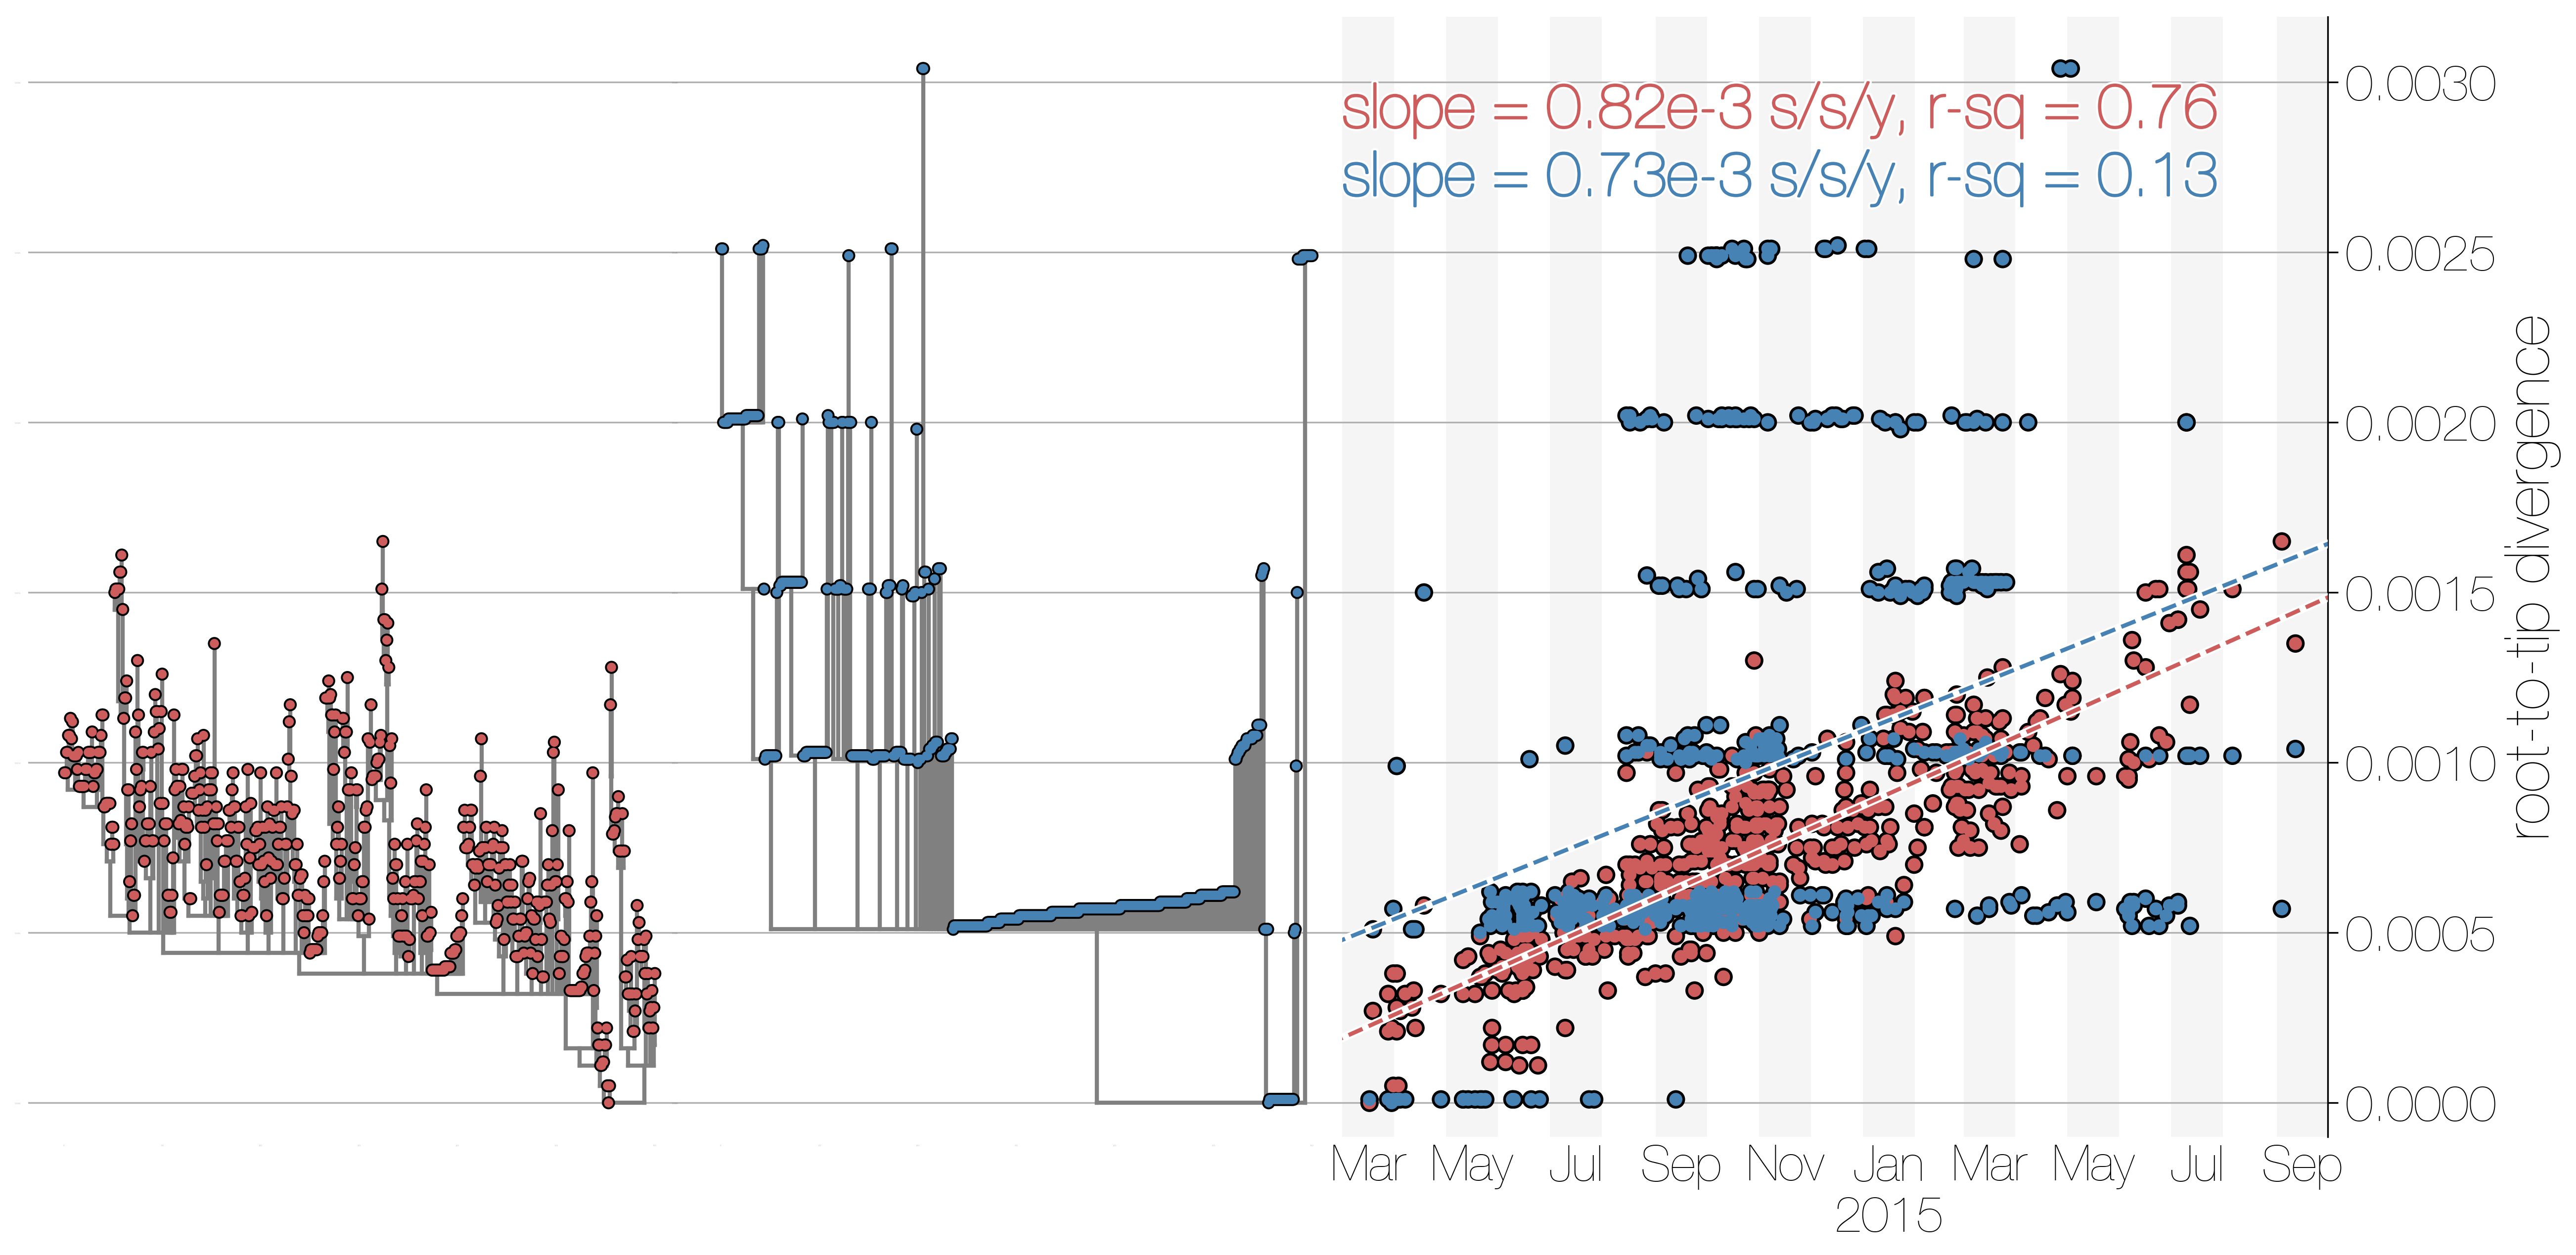
\includegraphics[width=0.75\textwidth]{supp_figures/sfig3_rtt.png}
	\caption{\textbf{Root to tip regression for maximum likelihood trees of genome (red) and GP (blue) sequences.}
  Linear regression of sequence collection dates against distance from the root gives evolutionary rate estimates (slope of the regression) at $0.82\times10^{-3}$ and $0.73\times10^{-3}$ substitutions per site per year, respectively.
  Despite similar rates the correlation between collection dates and divergence from root is far better using genomes ($r^{2}=0.76$) than GP sequences ($r^{2}=0.13$).
	}
	\label{rtt}
\end{figure}

\begin{figure}[h]
 \centering
	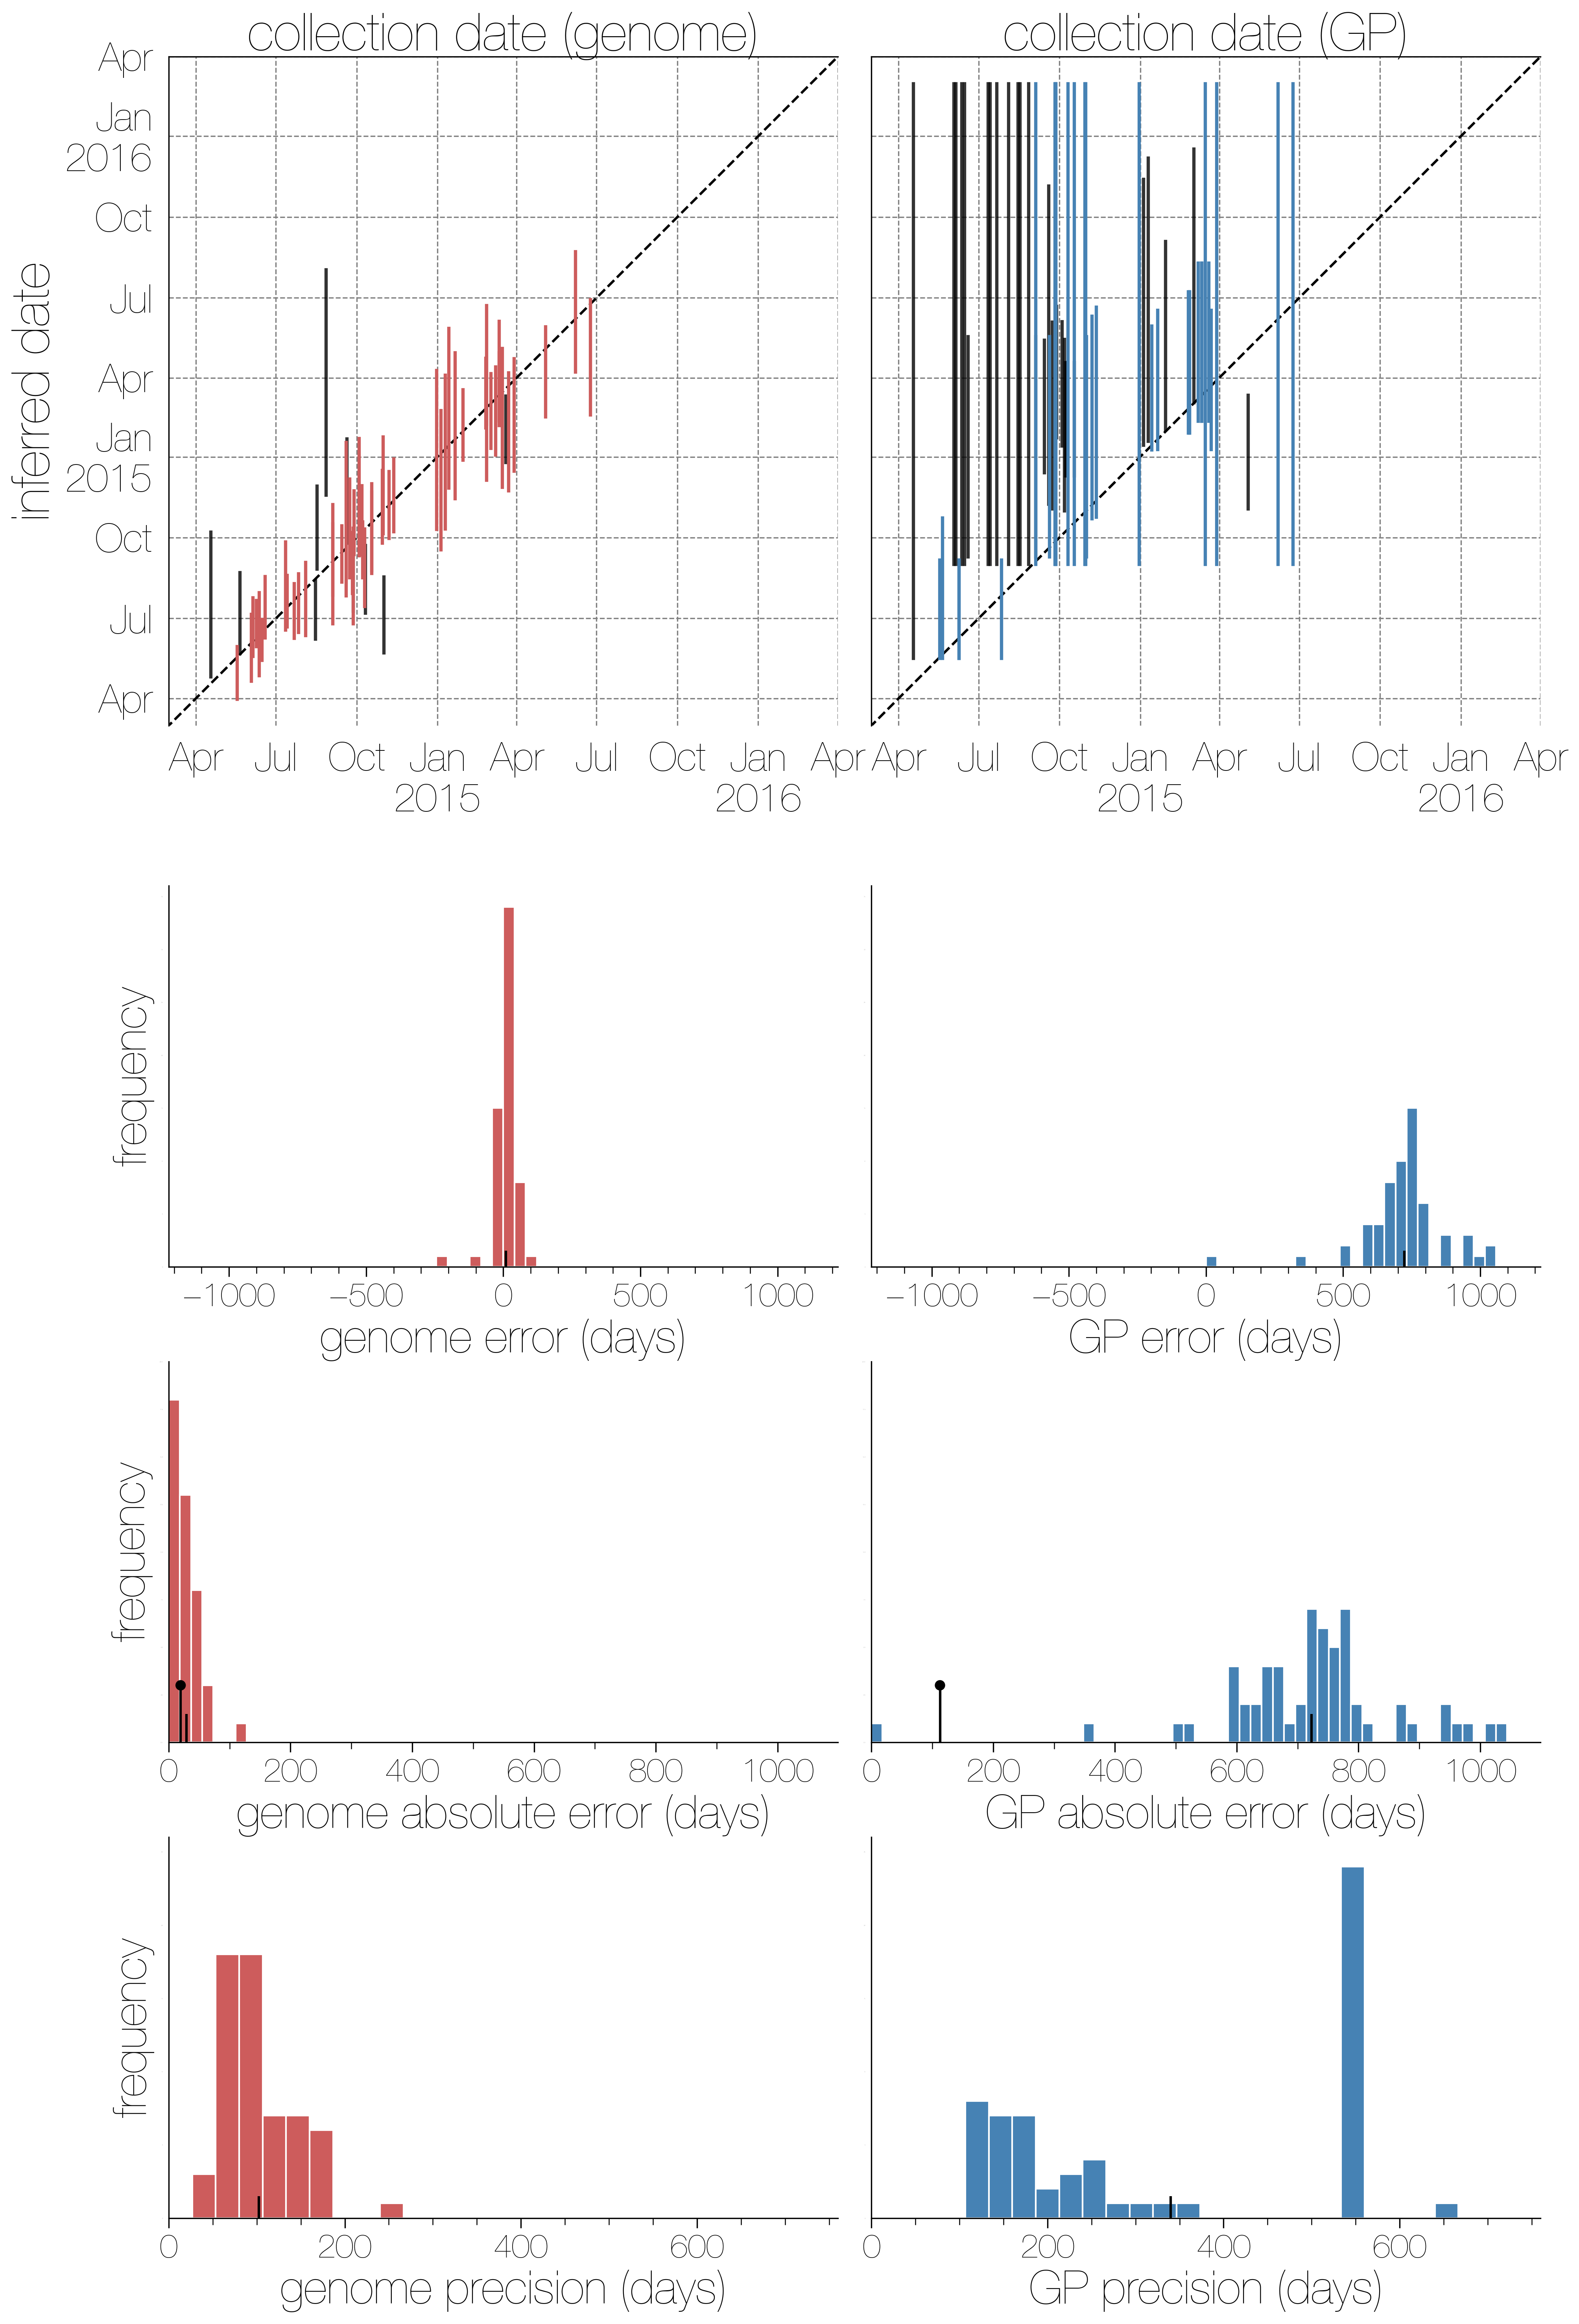
\includegraphics[width=0.75\textwidth]{supp_figures/sfig4_treetimeDates.png}
	\caption{\textbf{Maximum likelihood inference of masked tip dates from genomes (red, left) and GP sequences (blue, right) using TreeTime.}
  Vertical bars indicate the 95\% confidence interval for marginal reconstruction of masked tip dates plotted against their true dates.
  Tip dates where the 95\% confidence interval excludes the true value are shown in black.
	}
	\label{TTdates}
\end{figure}

\begin{figure}[h]
 \centering
	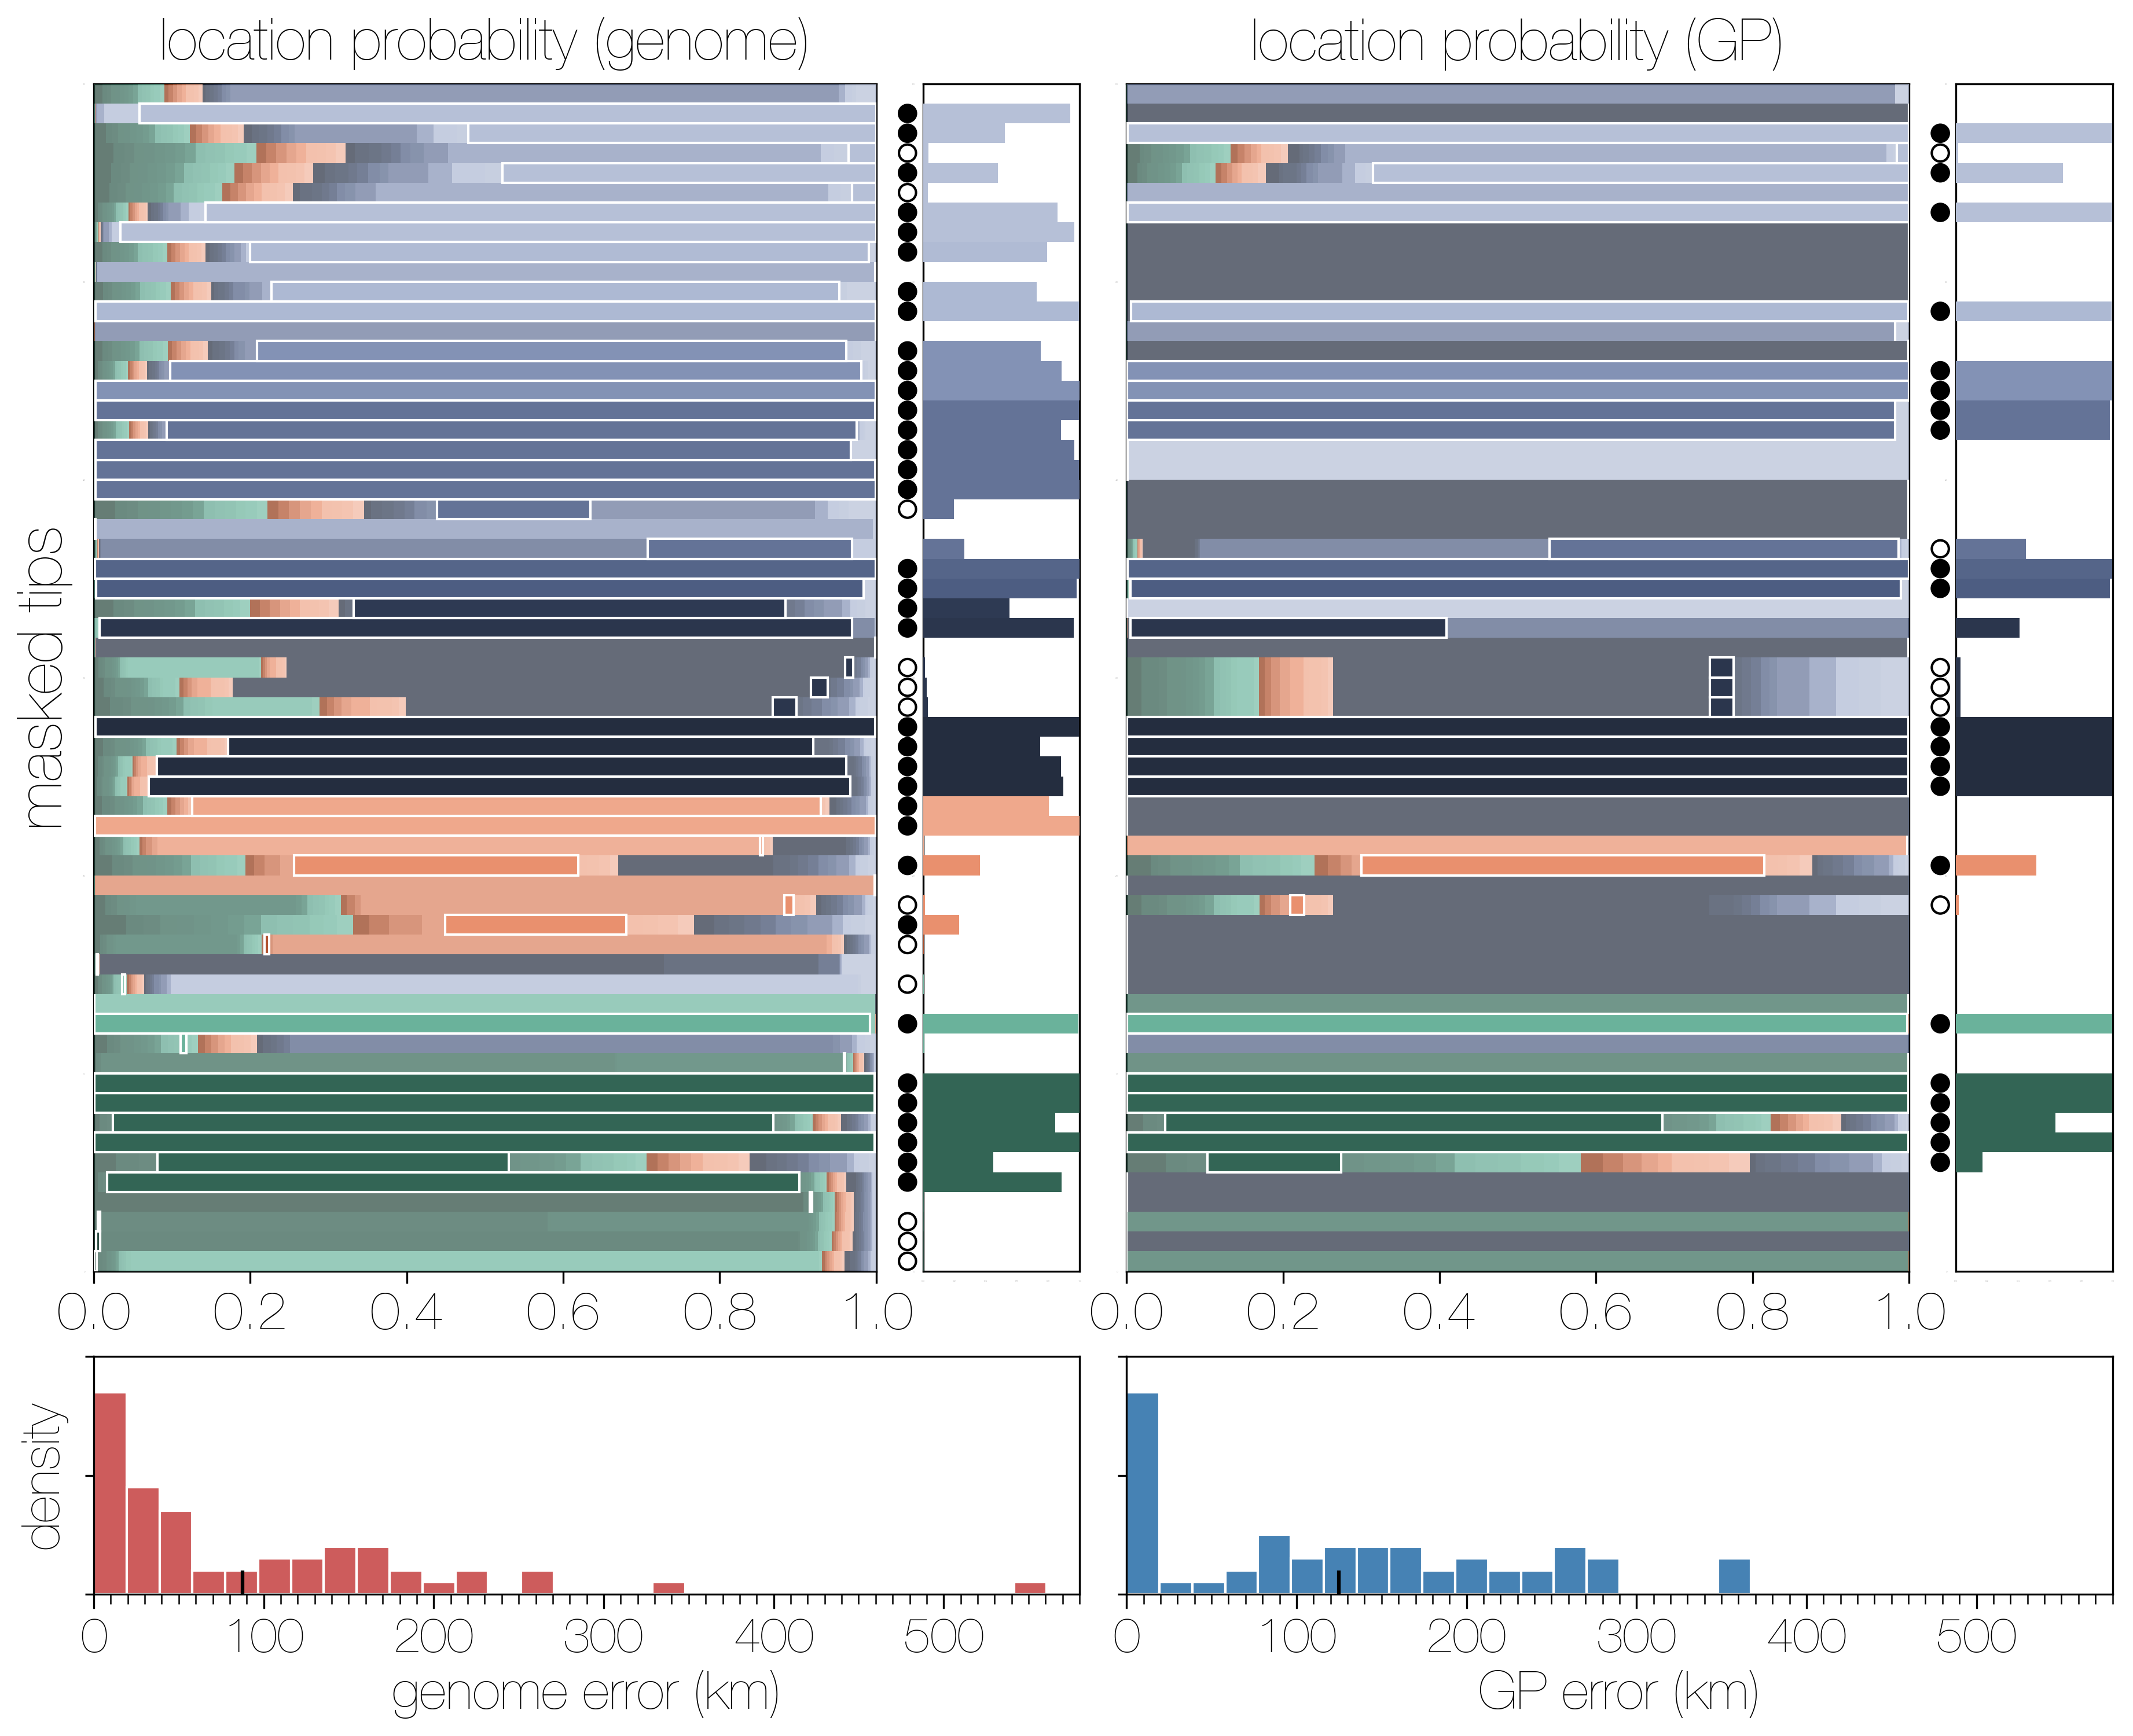
\includegraphics[width=0.75\textwidth]{supp_figures/sfig5_treetimeLocations.png}
	\caption{\textbf{Maximum likelihood inference of masked sequence location from genomes (left) and GP sequences (right) via a CTMC model implemented in TreeTime.}
  Horizontal bars indicate the posterior distribution of masked tip locations coloured by country (Sierra Leone in blue, Liberia in red, Guinea in green) and location (lighter colours indicate administrative divisions lying towards west of the country).
  The correct location of each tip is outlined in white with the smaller plot to the right showing only the probability of the correct location.
  Bars marked with an open circle indicate cases where the correct location is within the 95\% credible set and solid circles indicate cases where the location with the most probability is also the correct location.
  Genomes still perform better in terms of correct guess (0.432 probability that best guess location is true location for genomes versus 0.259 for GP), cross entropy (12012.800 nats for genome versus 24397.109 nats for GP) and mean probability-weighted great circle distance between true location population centroid and estimated location population centroid (87.568 km for genome versus 124.909 km for GP).
	}
	\label{TTlocations}
\end{figure}

\begin{figure}[h]
 \centering
	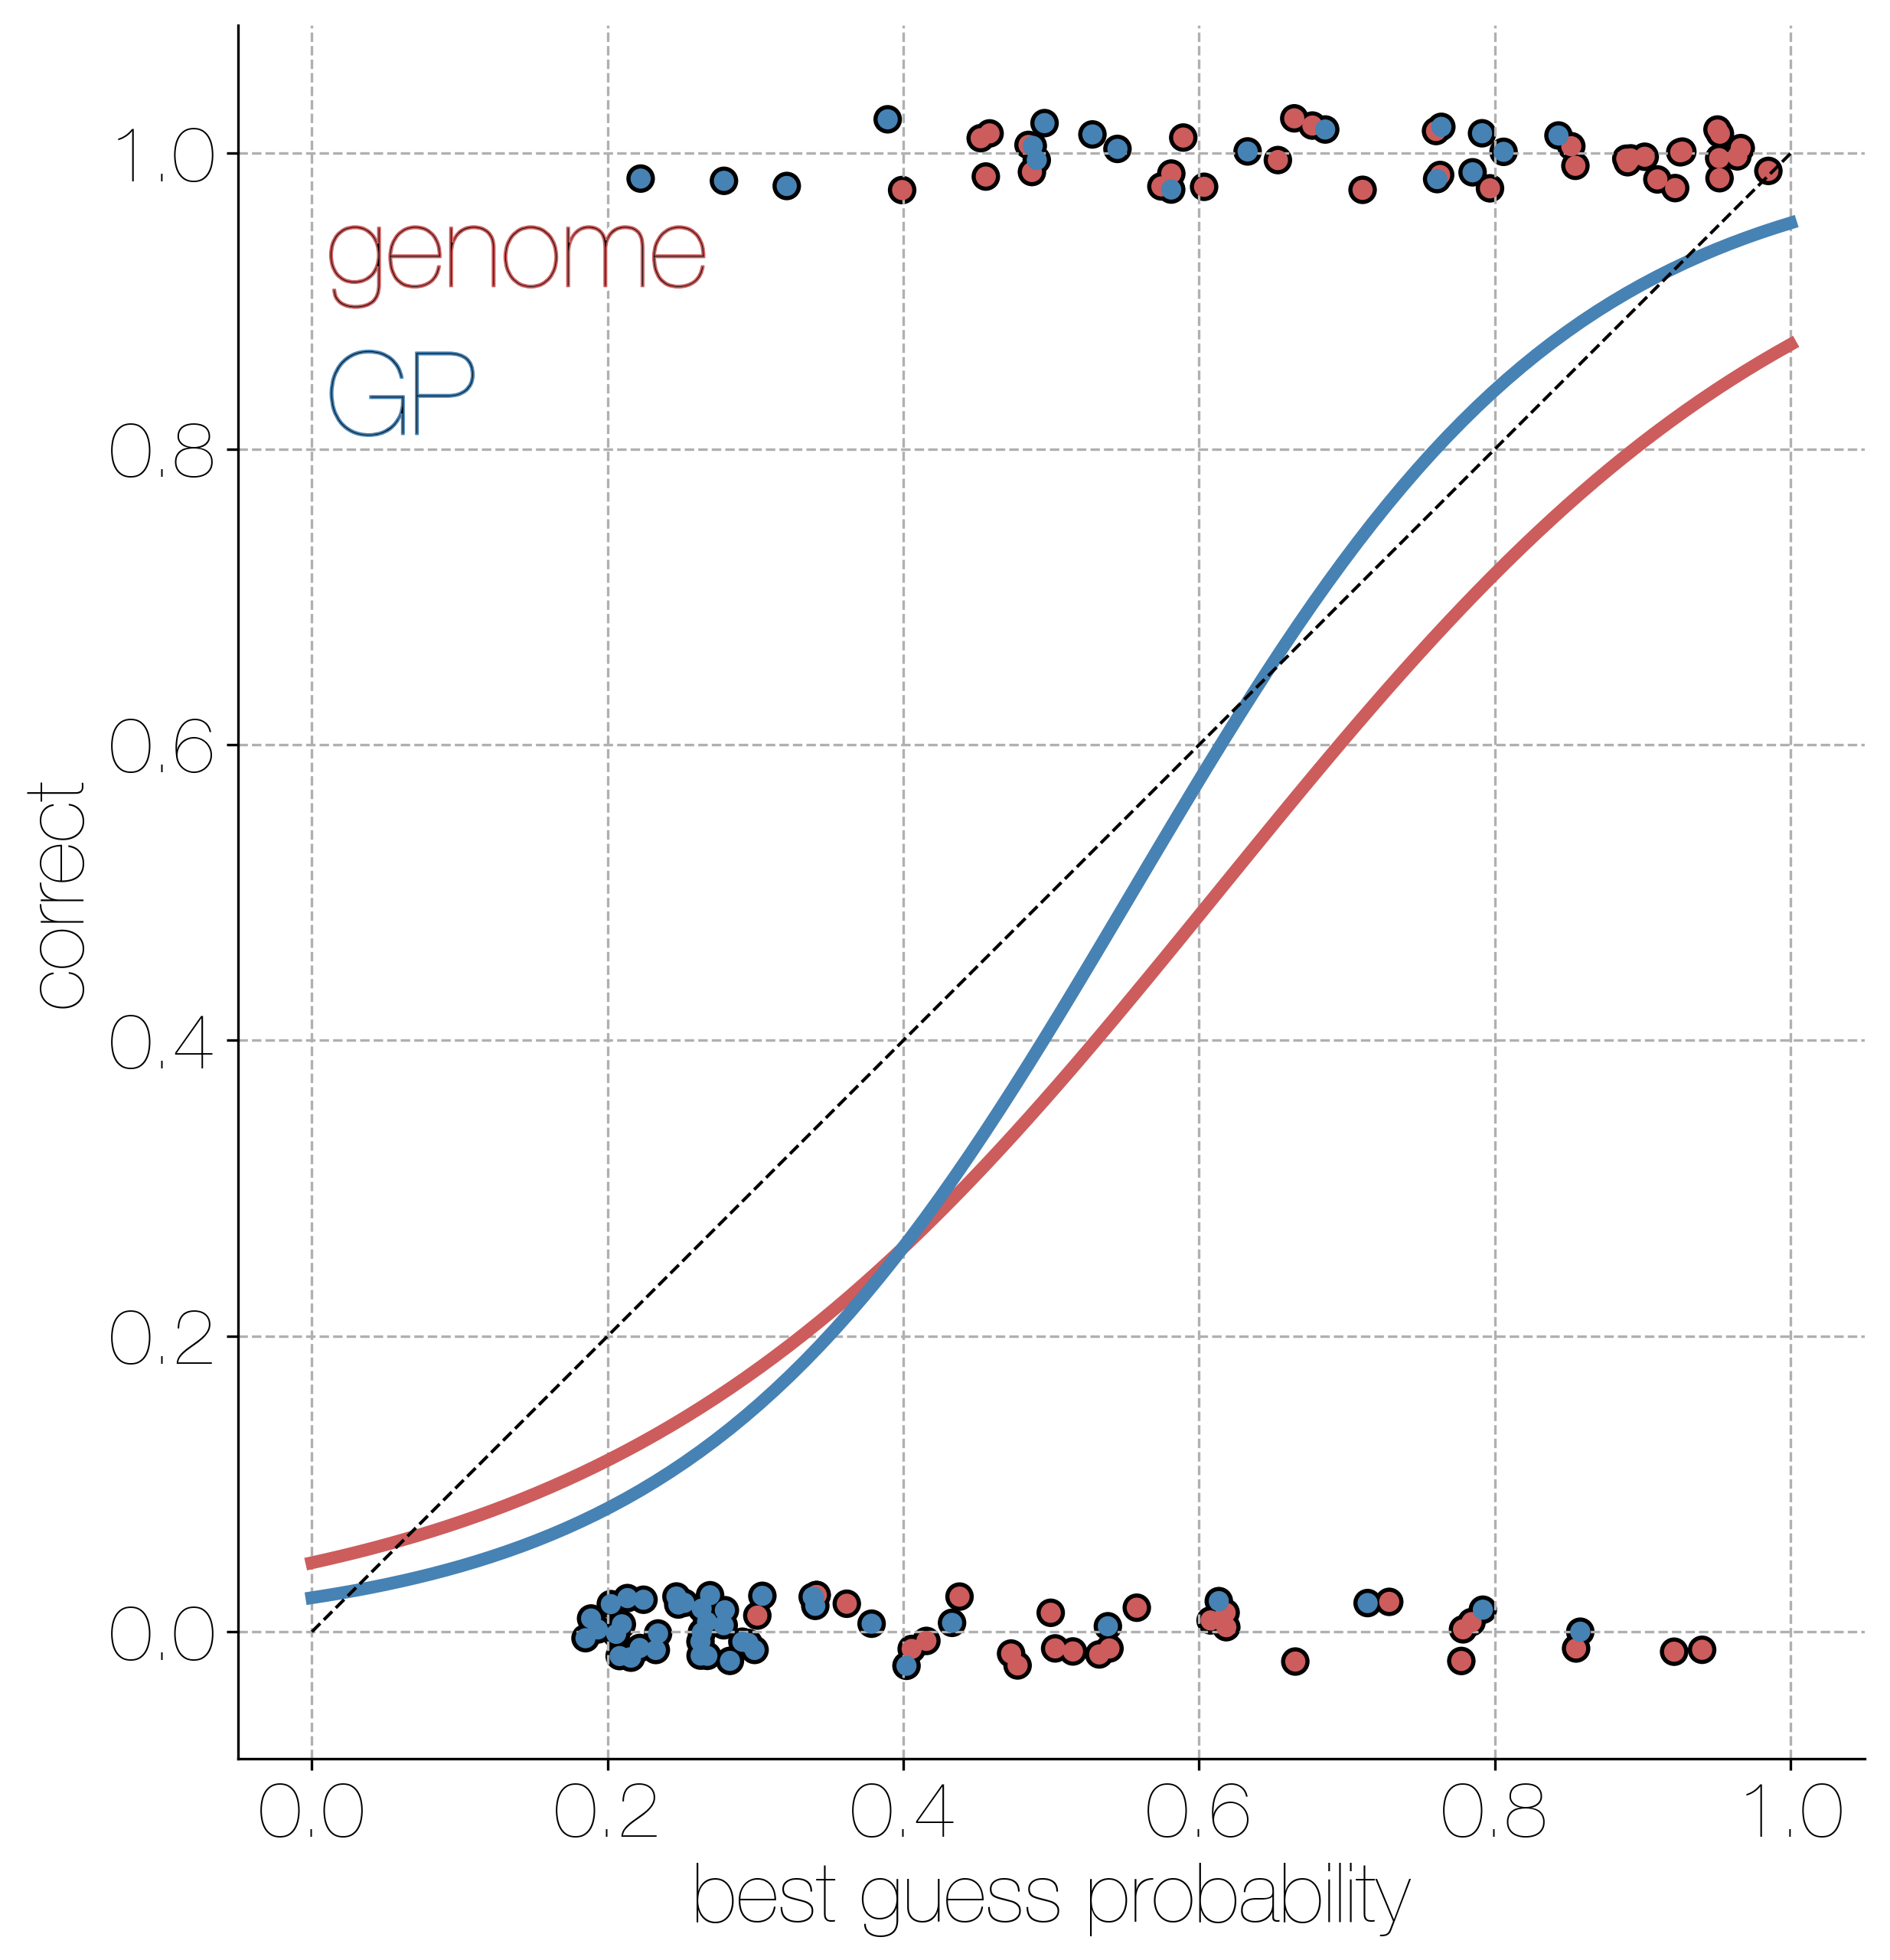
\includegraphics[width=0.75\textwidth]{supp_figures/sfig6_calibration.png}
	\caption{\textbf{Calibration curve for phylogeographic model informed with genome (red) and GP (blue) sequences.}
  Logistic regression of probability of the most likely location against whether it is correct or not for genome (red) and GP (blue) sequences with jitter introduced along the y axis to make points discernible.
  Overall performance of the phylogeographic model is comparable between genome and GP sequences as indicated by sigmoid curves matching the 1-to-1 dotted line.
	}
	\label{calibration}
\end{figure}

\begin{figure}[h]
 \centering
  \subfloat{
  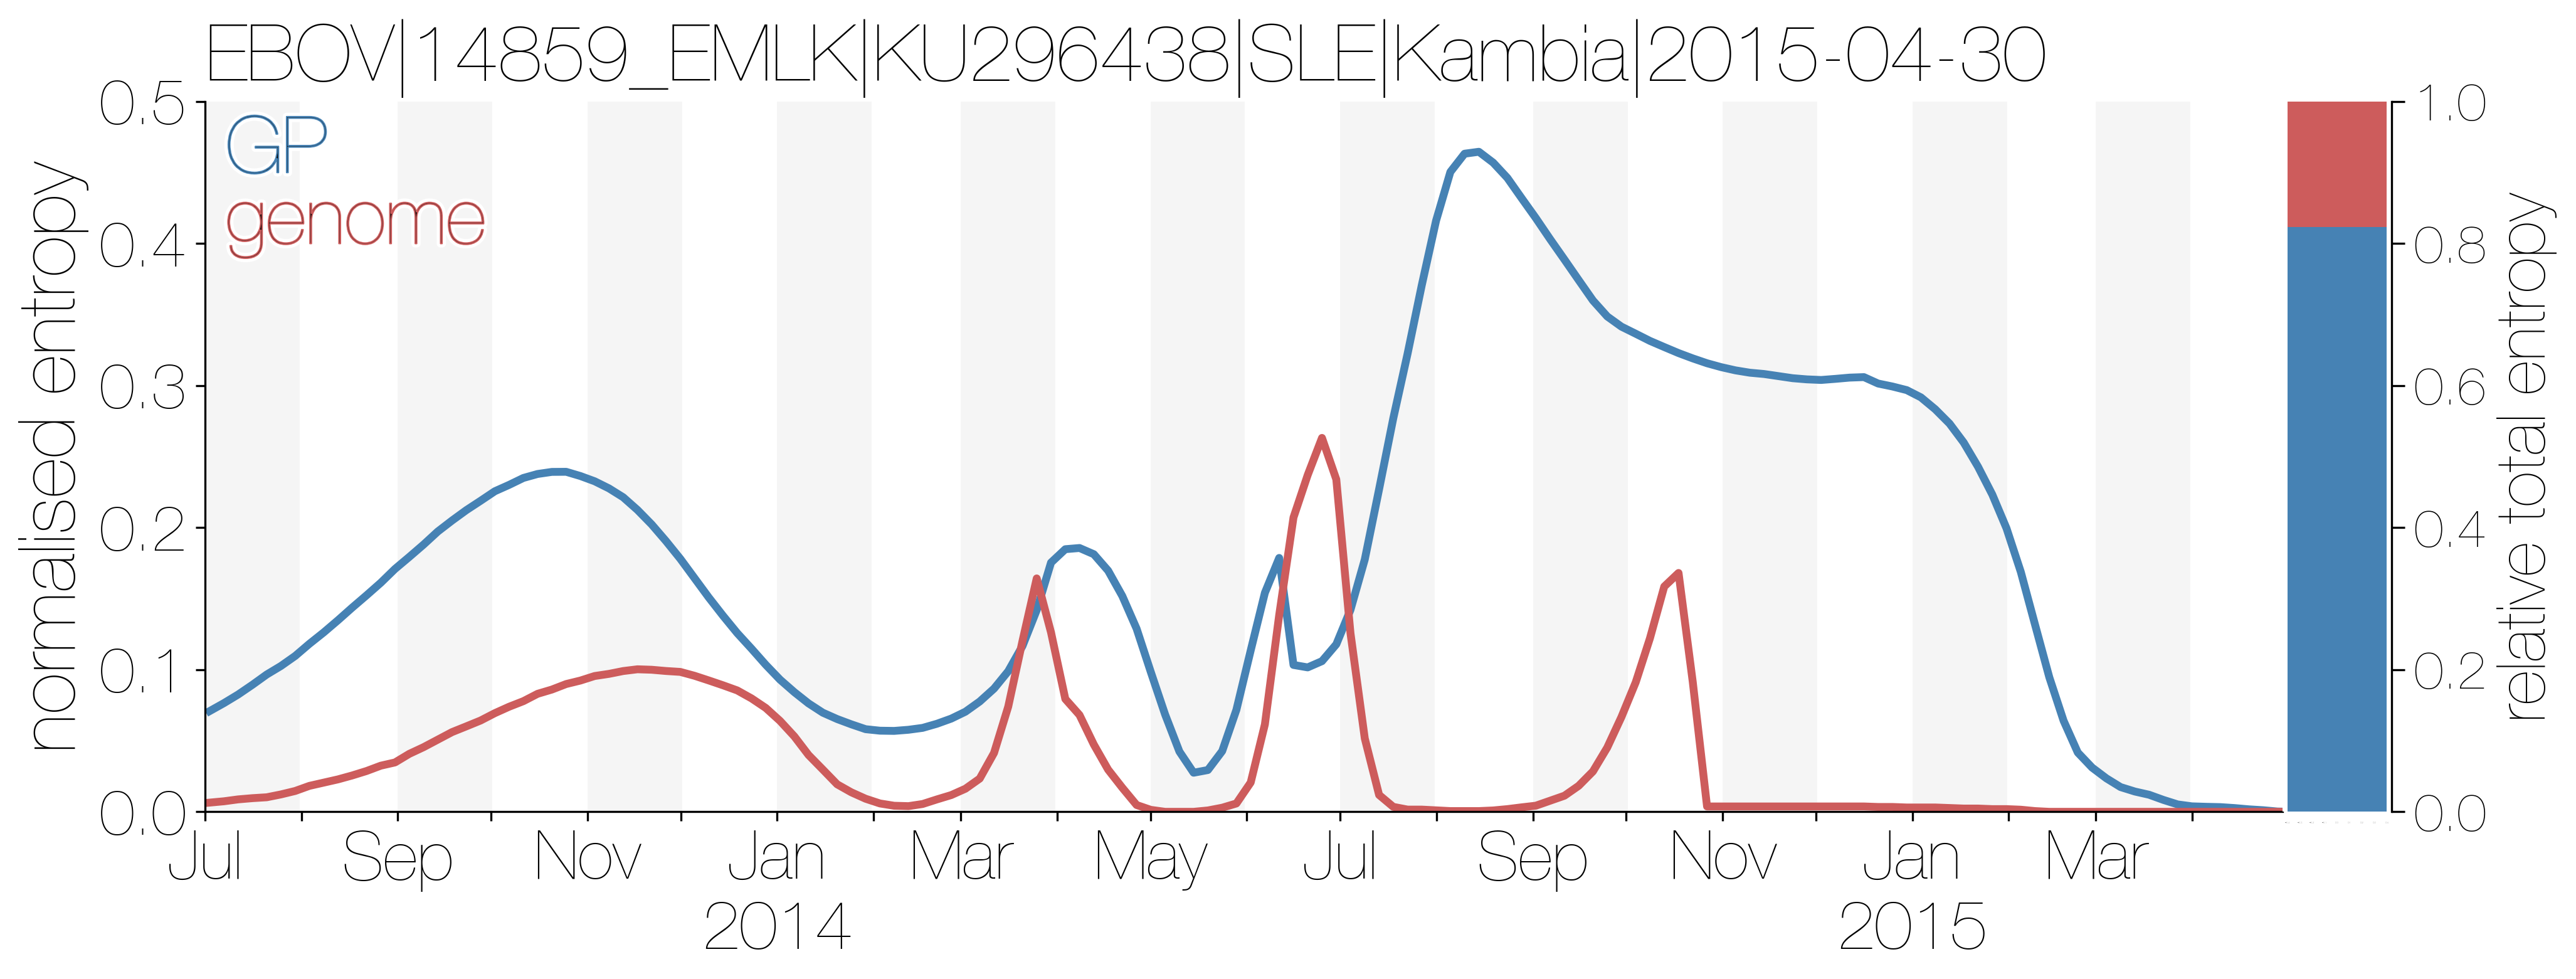
\includegraphics[width=0.45\textwidth]{supp_figures/sfig7A_locationEntropy.png}
  }
  \subfloat{
  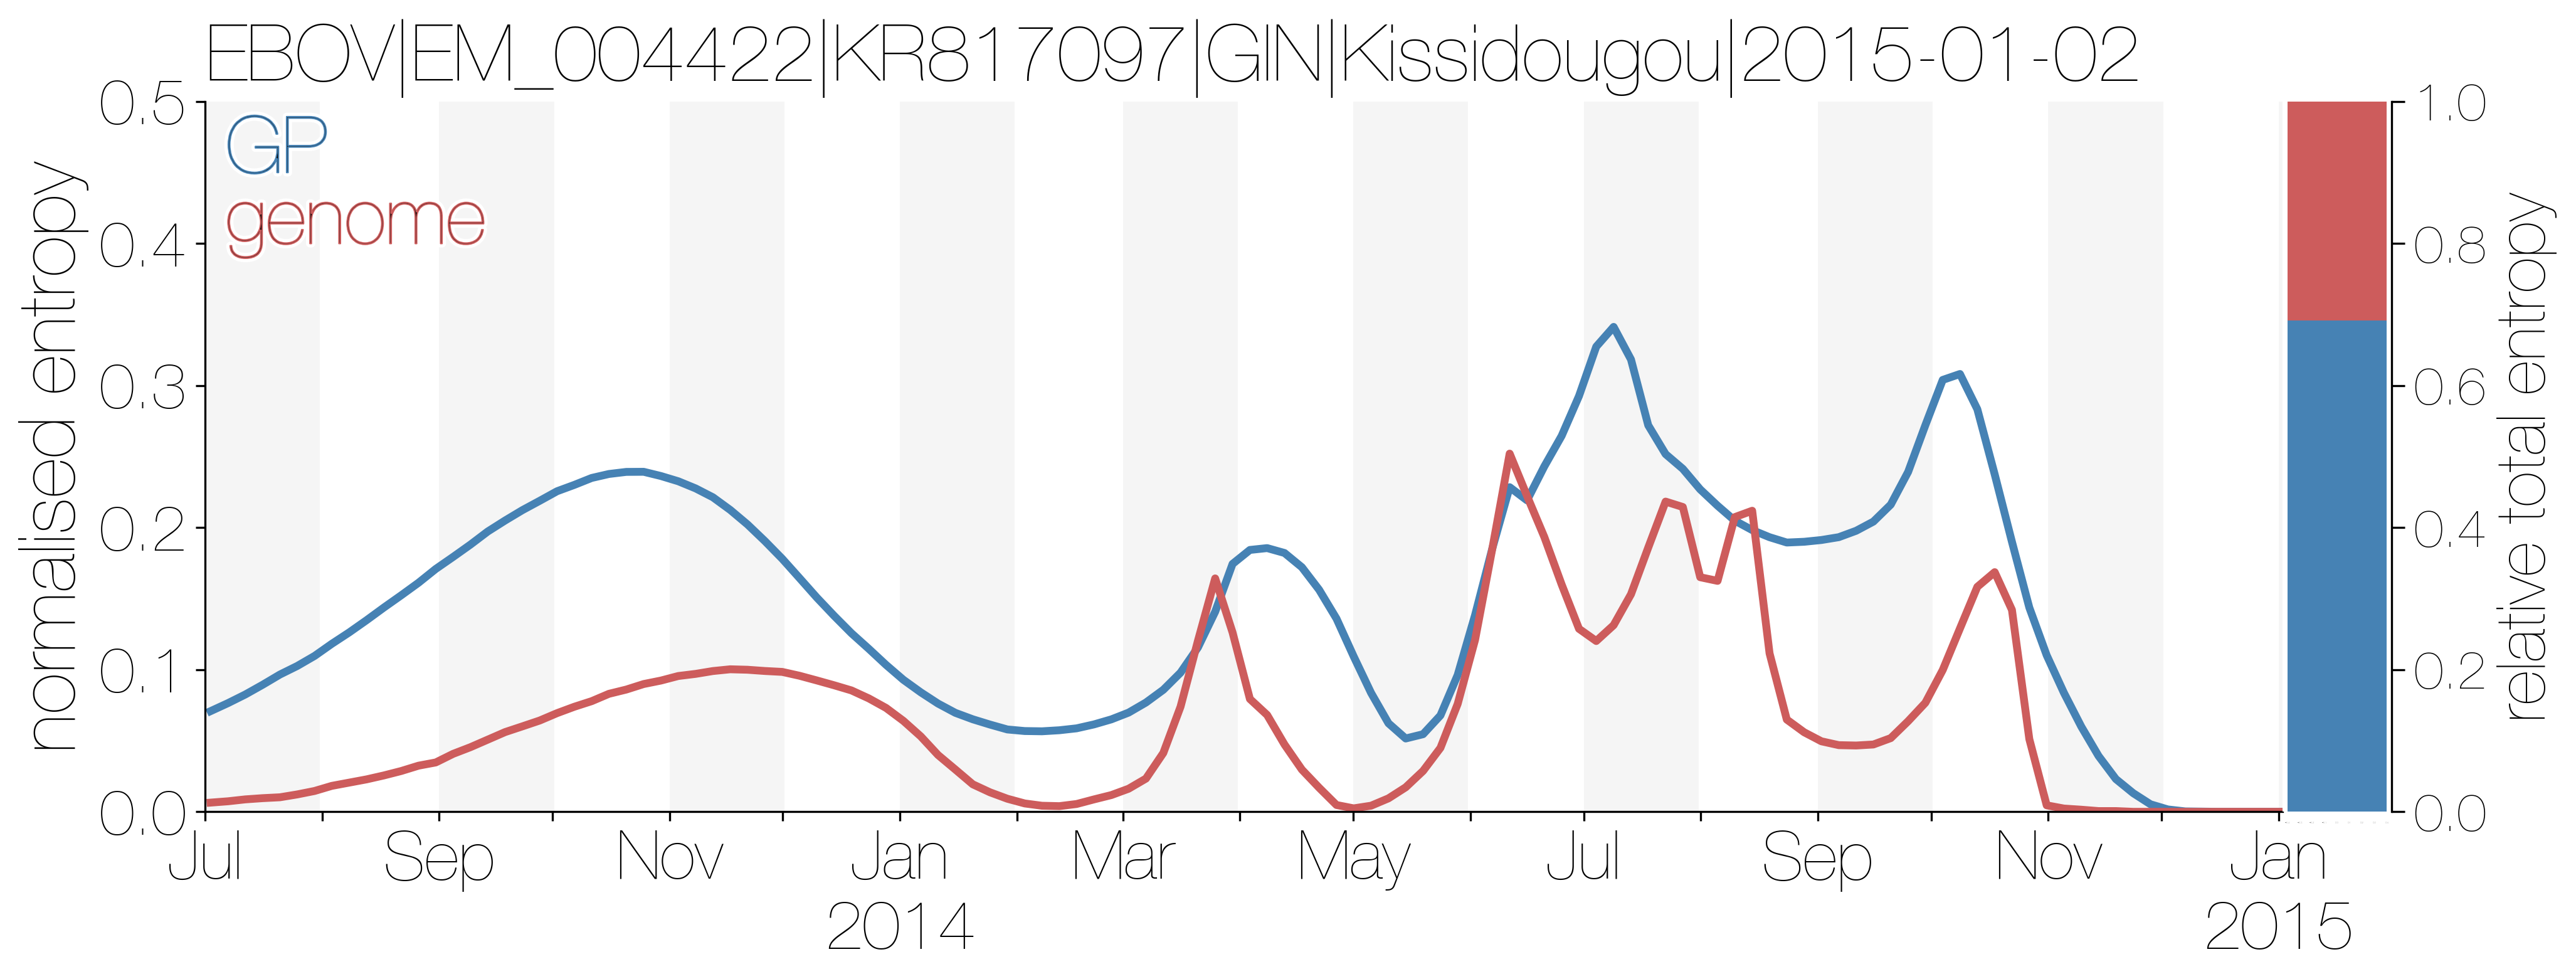
\includegraphics[width=0.45\textwidth]{supp_figures/sfig7B_locationEntropy.png}
  }
  \\
  \subfloat{
  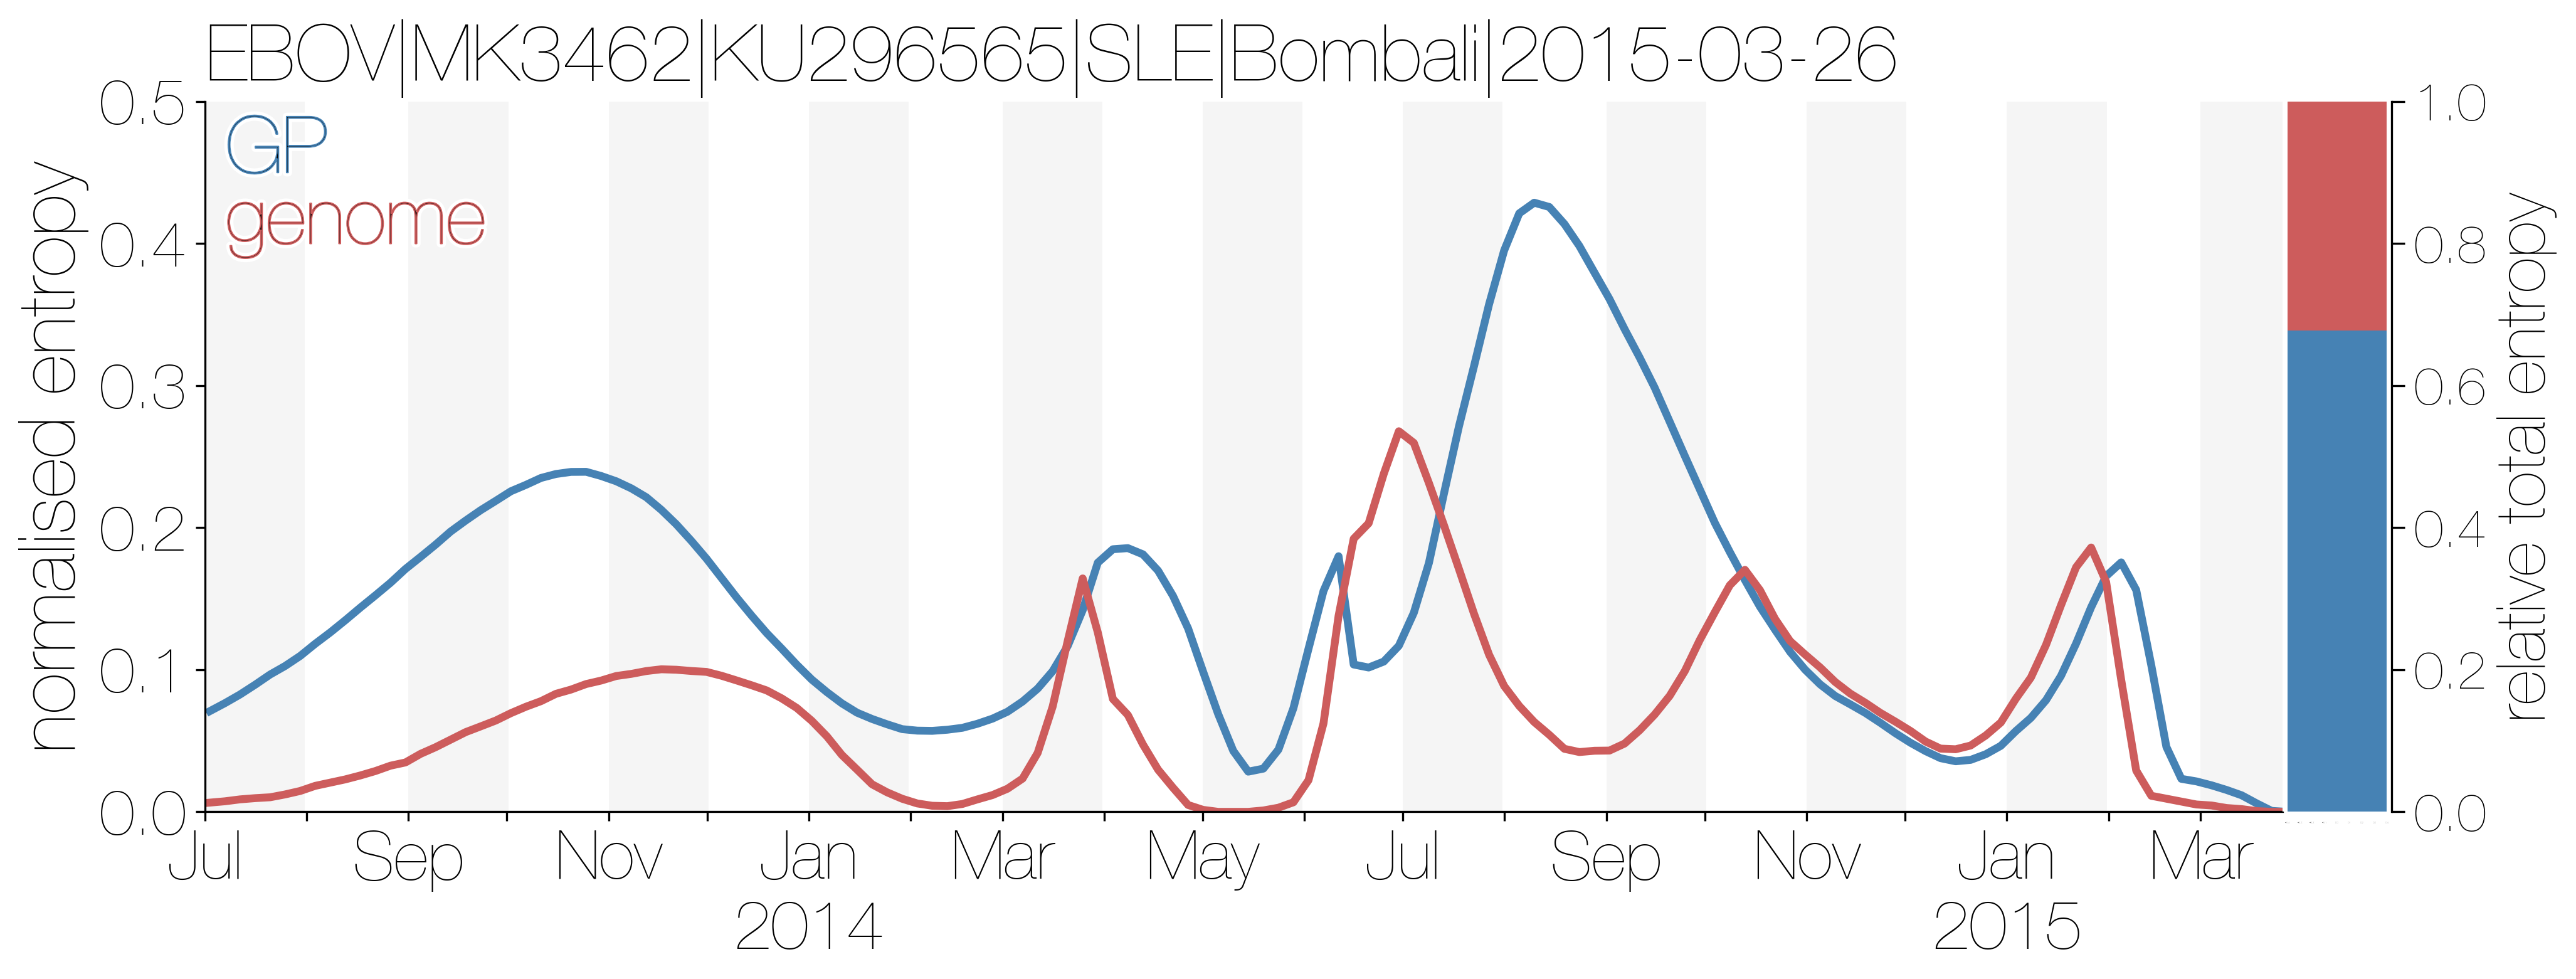
\includegraphics[width=0.45\textwidth]{supp_figures/sfig7C_locationEntropy.png}
  }
  \subfloat{
  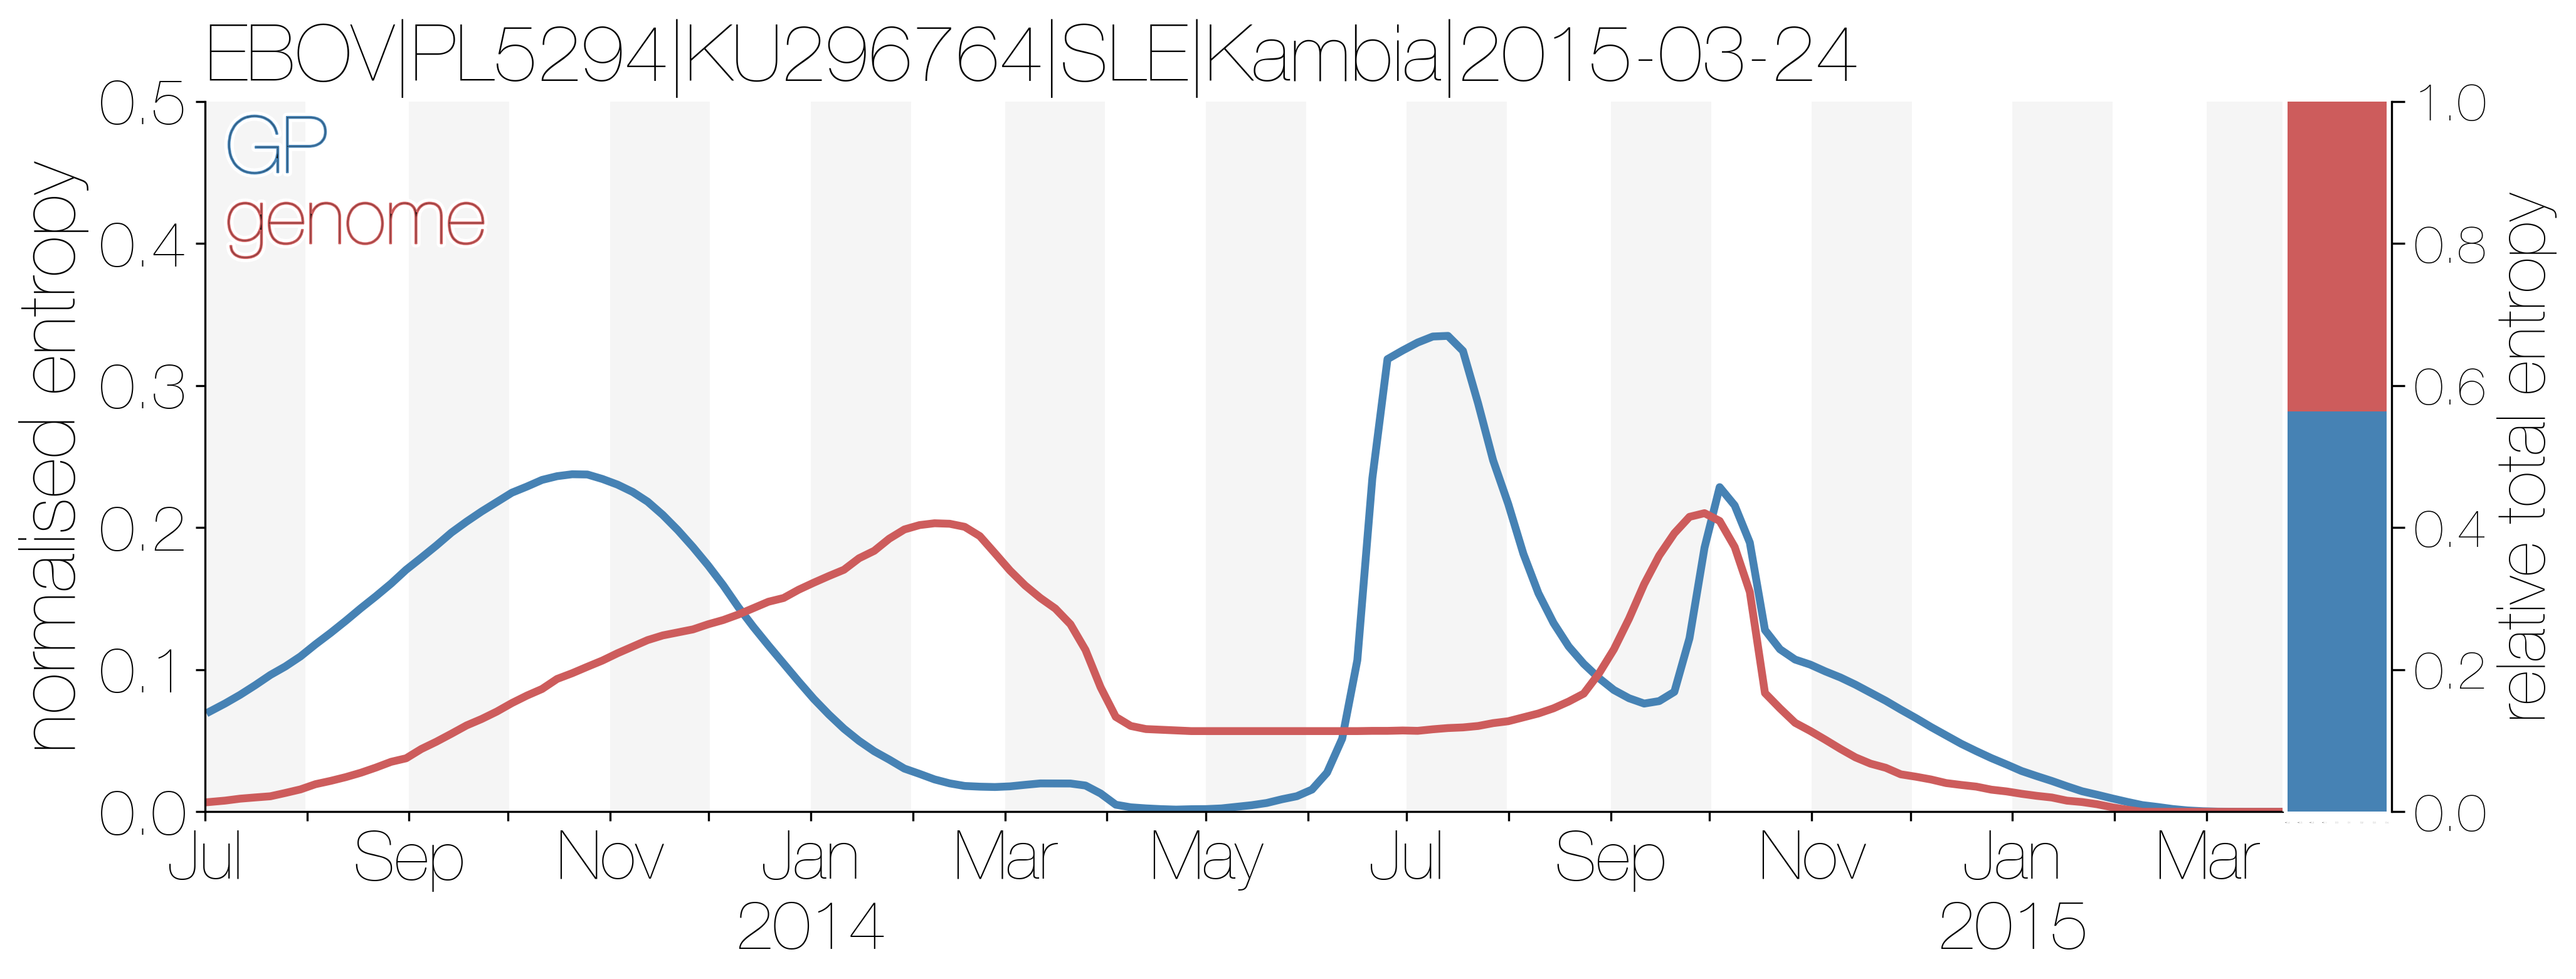
\includegraphics[width=0.45\textwidth]{supp_figures/sfig7D_locationEntropy.png}
  }
  \caption{\textbf{Entropies of posterior ancestral location reconstruction from genomes (red) and GP sequences (blue) for four tips.}
  Ancestral state reconstructions from genomes typically have lower entropies relative to reconstructions derived from GP sequences indicating better certainty in location assignment at any given time.
  Red and blue bars at the end of the plot indicate relative cumulative entropies of genome and GP sequence reconstructions, respectively.
  }
	\label{trace_entropy}
\end{figure}

\begin{figure}[h]
 \centering
	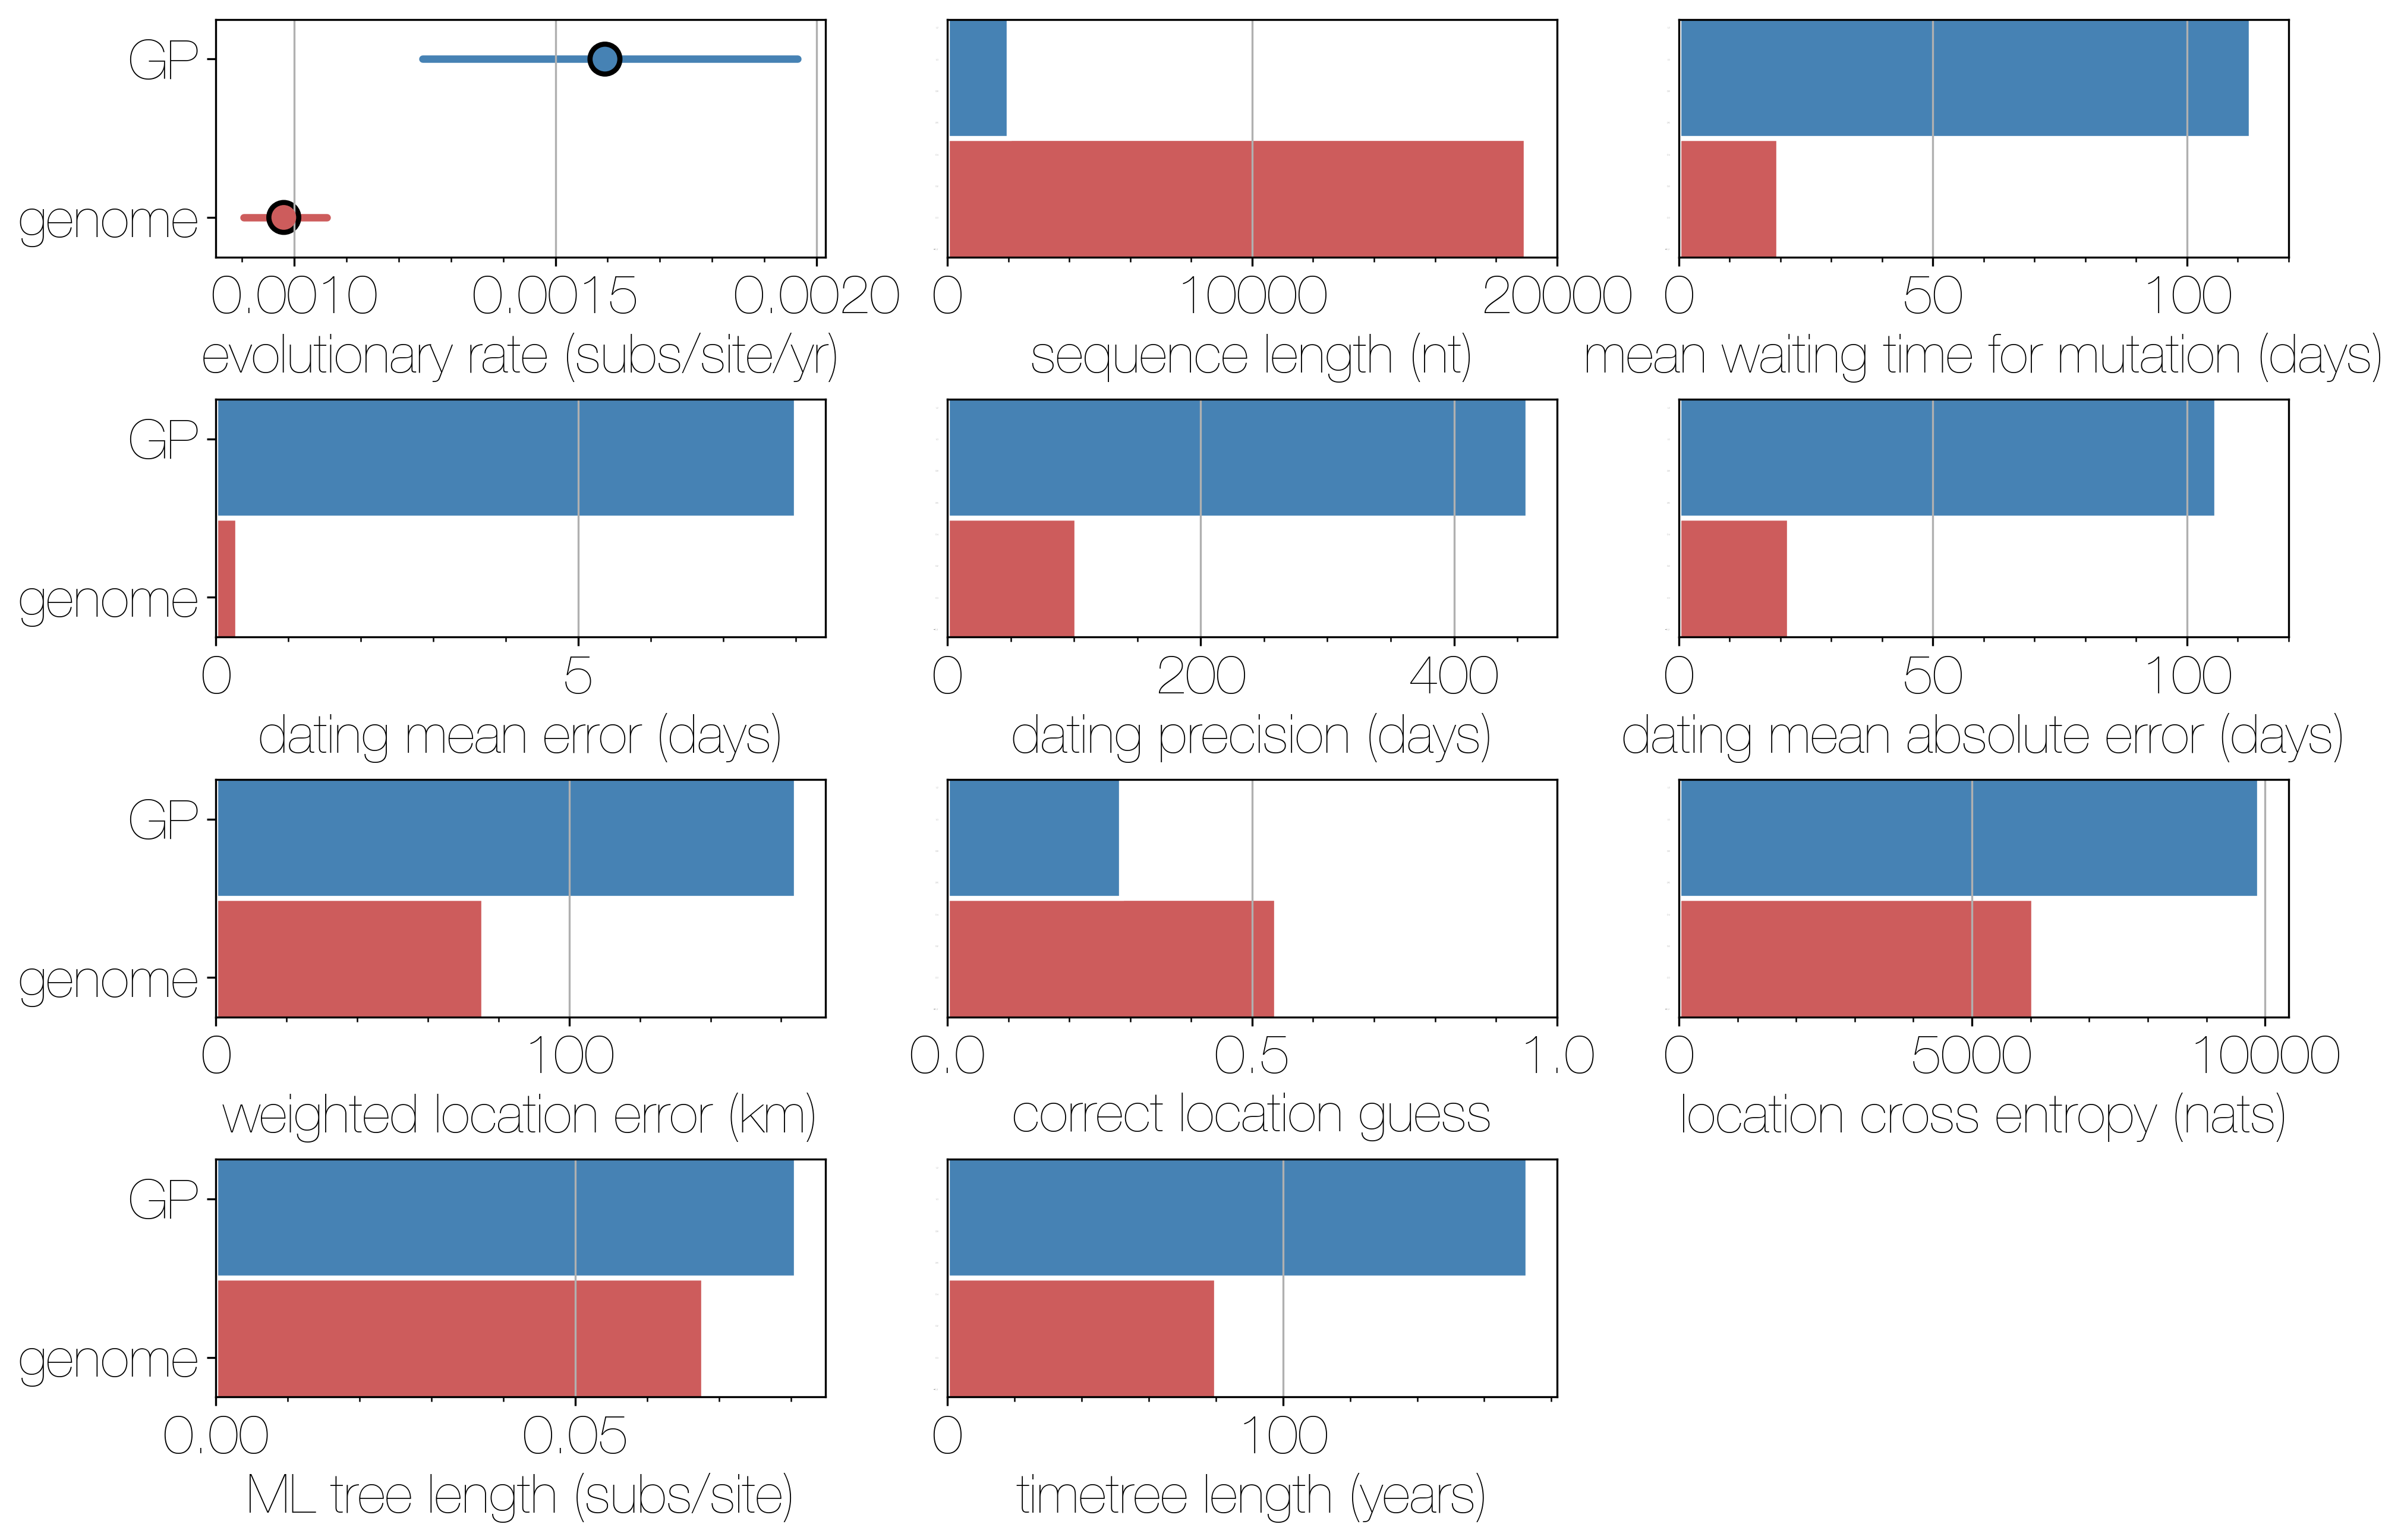
\includegraphics[width=0.75\textwidth]{supp_figures/sfig8_summary.png}
	\caption{\textbf{Summary of statistics reported in this study.}
  Each cell shows the difference between genome (red, bottom of cell) and GP (blue, top of cell) data for various statistics reported in this study.
  Descriptions for each statistic are given at the bottom of the cell near the x-axis.
	}
	\label{summary}
\end{figure}

\begin{figure}[h]
 \centering
  \subfloat{
  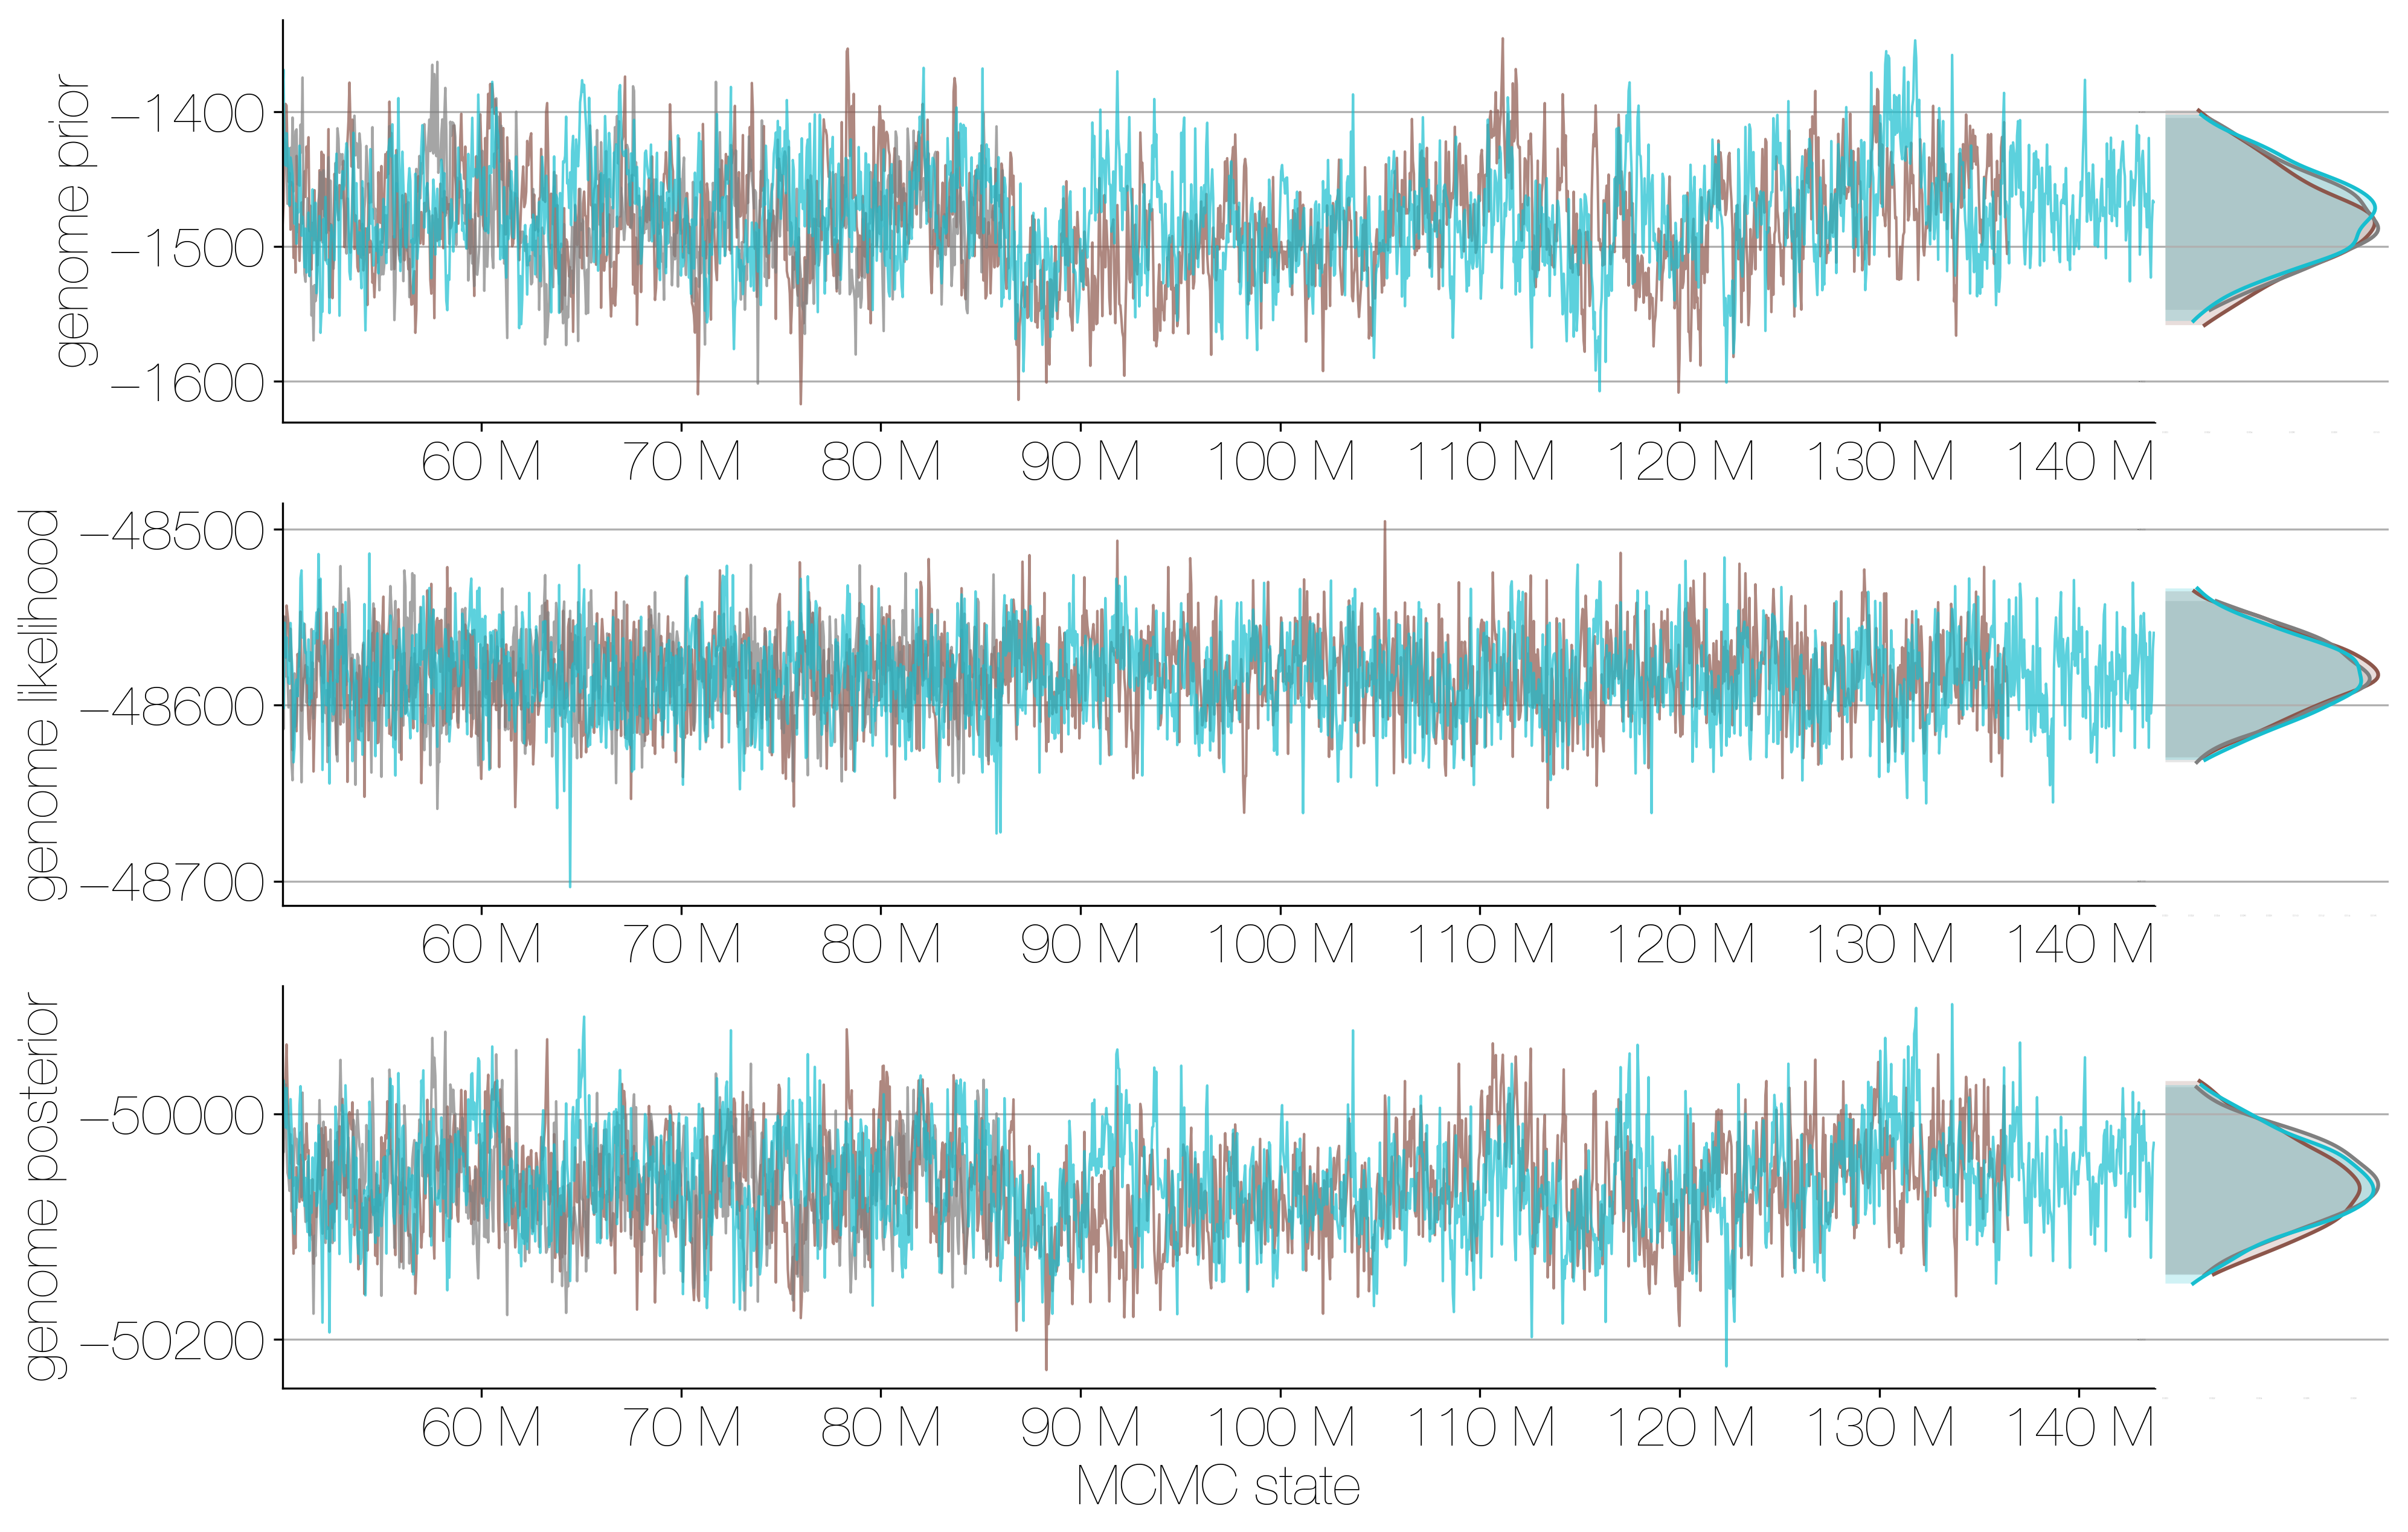
\includegraphics[width=0.65\textwidth]{supp_figures/sfig9A_genome_mcmc.png}
  }\\
  \subfloat{
  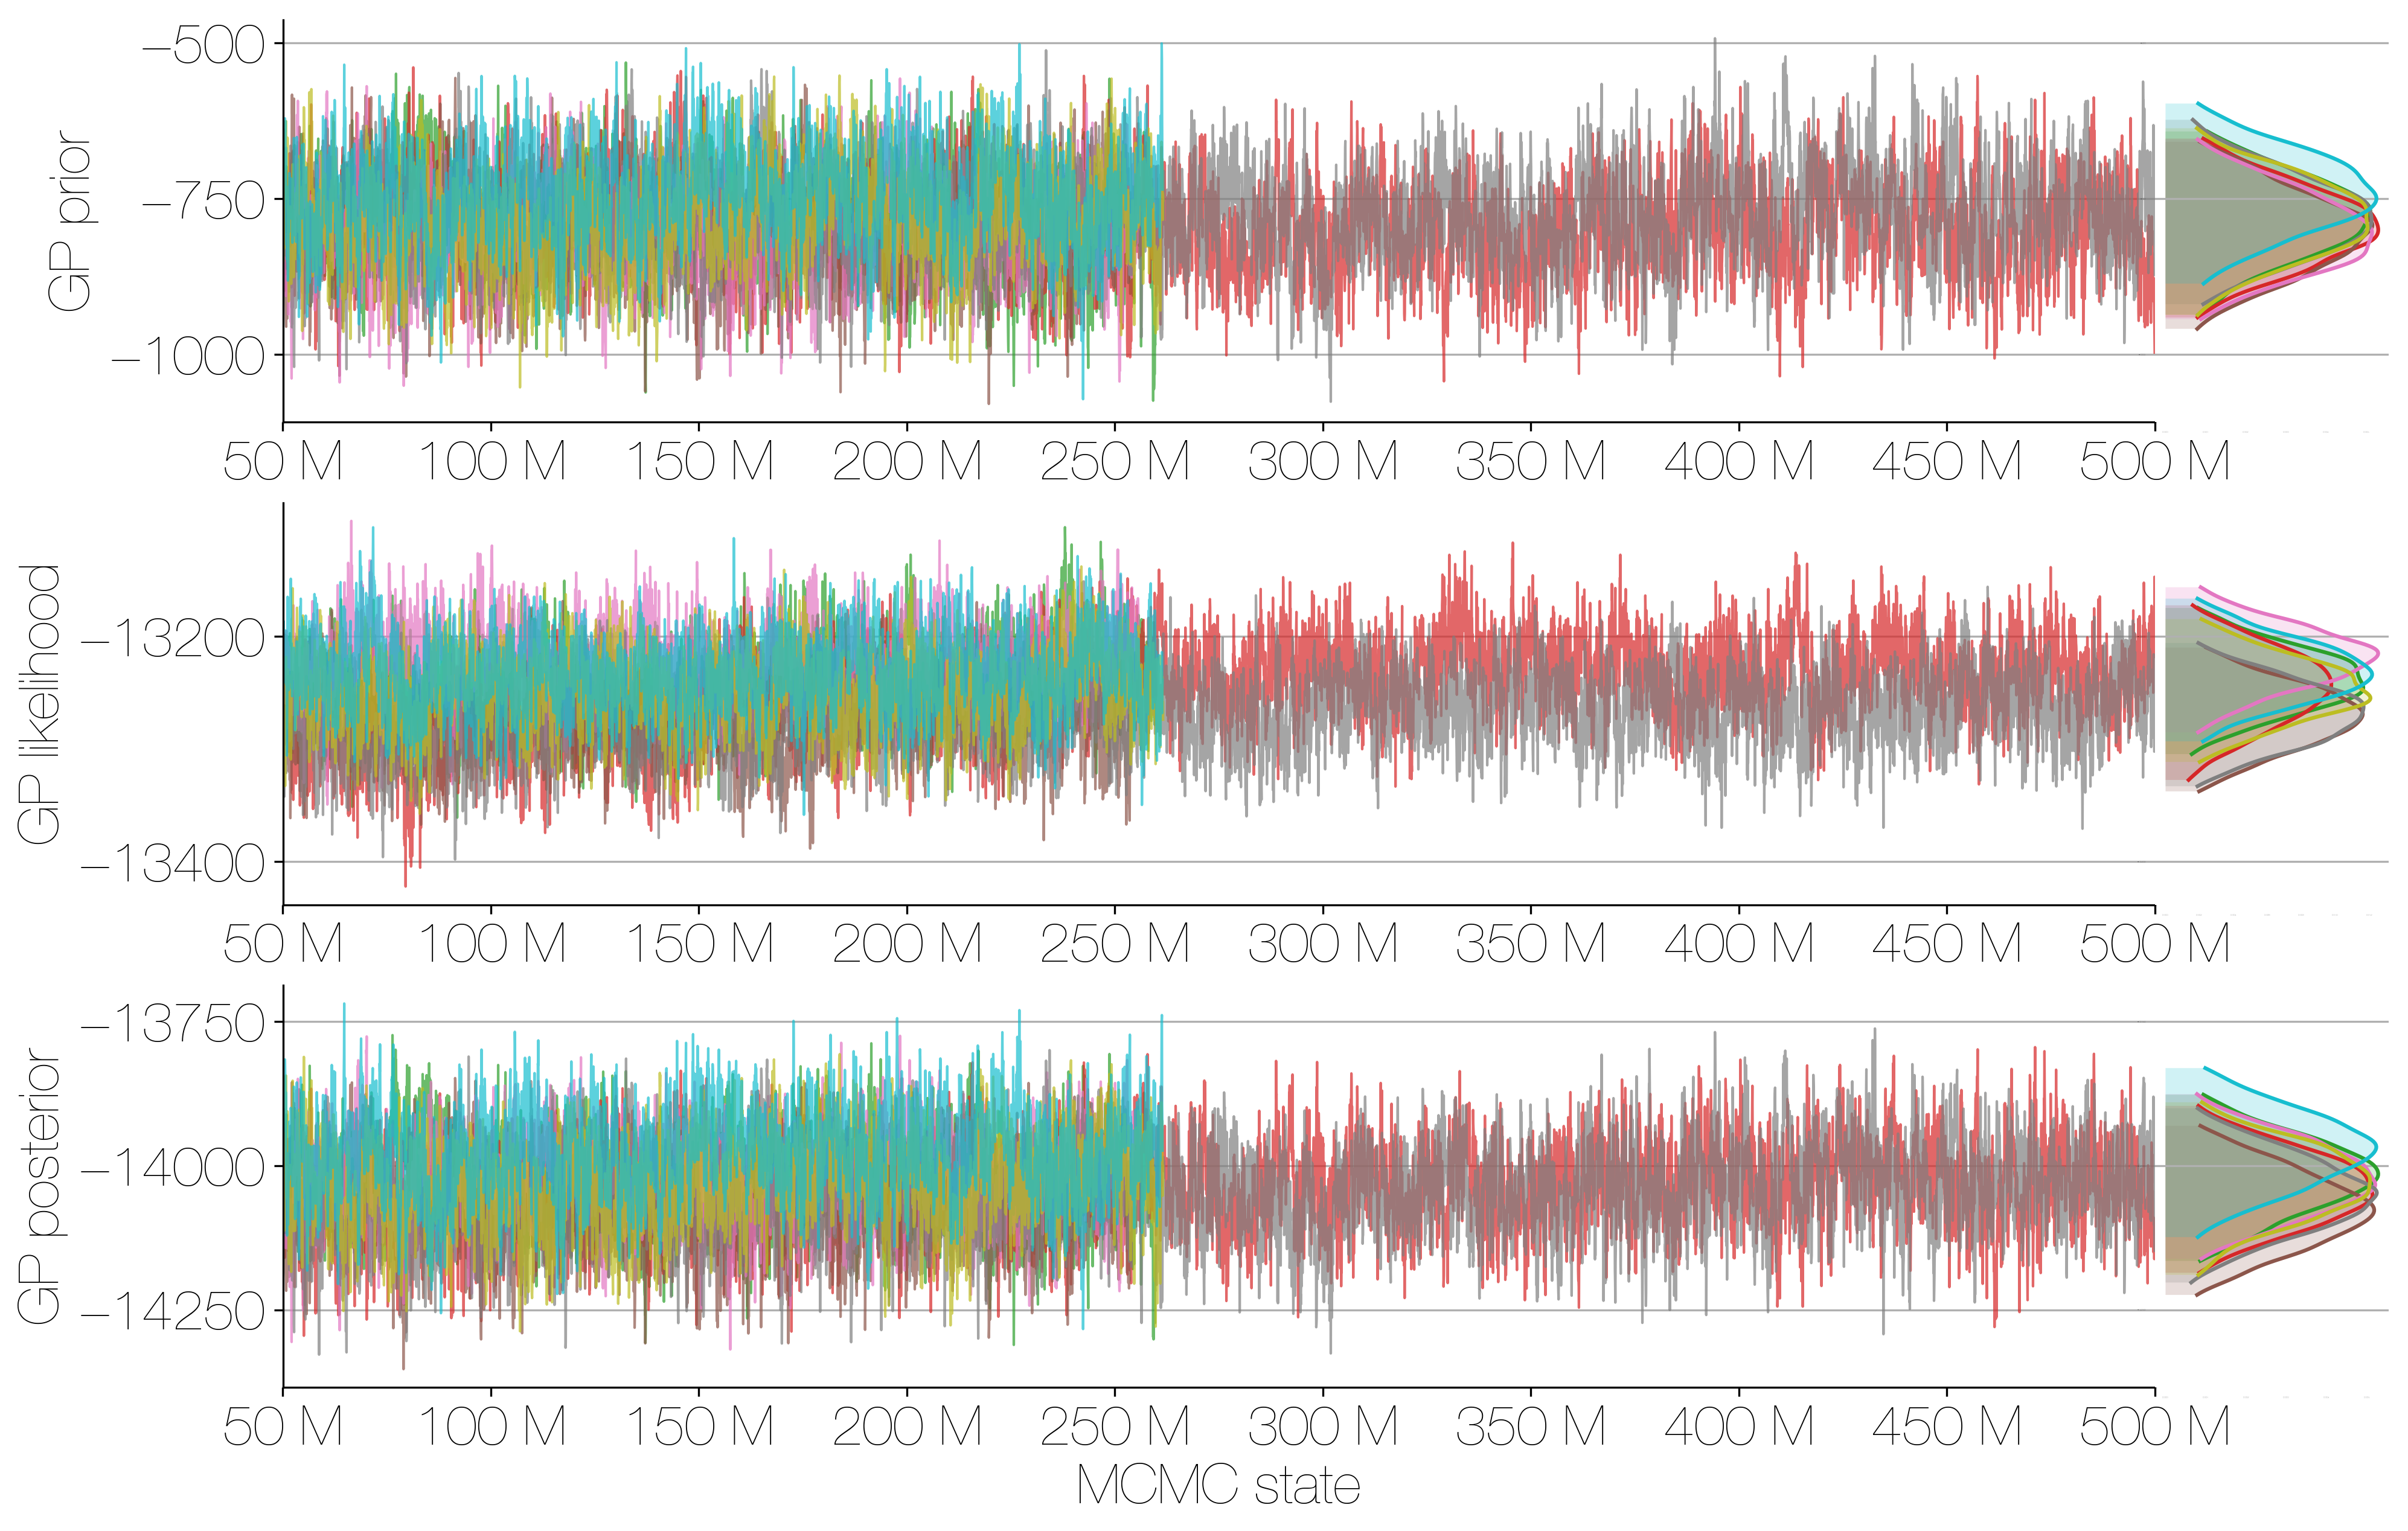
\includegraphics[width=0.65\textwidth]{supp_figures/sfig9B_gp_mcmc.png}
  }
  \\
  \caption{\textbf{MCMC traces of prior, likelihood and joint (referred to as posterior) probabilities.}
  Post-burnin MCMC samples of prior, likelihood and joint probabilities for genome data (total of three chains, top) and GP data (total of seven chains, bottom) with kernel density estimates of each chain displayed on the right.
  }
	\label{mcmc}
\end{figure}

\end{document}
